%%-----------------------------------------------------------------------------
%%
%%                                   Sean Mauch
%%                       California Institute of Technology
%%                         @ 1995-2004 No Rights Reserved
%%
%%-----------------------------------------------------------------------------

\flushbottom

%% CONTINUE: introduce curves, contours, particularly about infinity.
%% CONTINUE: add section labels to Exercises...


%%============================================================================
%%============================================================================
\chapter{Analytic Functions}

Students need encouragement. So if a student gets an answer right, 
tell them it was a lucky guess. That way, they develop a good, lucky feeling.%
\footnote{Quote slightly modified.}

\begin{flushright}
  -Jack Handey
\end{flushright}

%%============================================================================
\section{Complex Derivatives}
\index{complex derivative}



\paragraph{Functions of a Real Variable.}
The derivative of a function of a real variable is
\[
\frac{\dd}{\dd x} f(x) = \lim_{\Delta x \to 0} \frac{f(x+\Delta x)-f(x)}{\Delta x}.
\]
If the limit exists then the function is differentiable at the point $x$.
Note that $\Delta x$ can approach zero from above or below.  The limit 
cannot depend on the direction in which $\Delta x$ vanishes.

Consider $f(x) = |x|$.  The function is not differentiable at $x = 0$ since
\[
\lim_{\Delta x \to 0^+} \frac{|0 + \Delta x| - |0|}{\Delta x} = 1
\]
and
\[
\lim_{\Delta x \to 0^-} \frac{|0 + \Delta x| - |0|}{\Delta x} = -1.
\]



\paragraph{Analyticity.}
The \textit{complex derivative}, (or simply \textit{derivative} 
if the context is clear), is defined, 
\index{complex derivative}
\index{derivative!complex}
\[ 
\frac{\dd}{\dd z} f(z) = \lim_{\Delta z \to 0}\frac{f(z + \Delta z) - f(z)}{\Delta z}.
\]
The complex derivative exists if this limit exists.  This means that the 
value of the limit is independent of the manner in which $\Delta z \to 0$.  
If the complex derivative exists at a point, then we say that the function
is \textit{complex differentiable} there.

A function of a complex variable is \textit{analytic} 
\index{analytic}
at a point $z_0$ if the complex derivative exists in a neighborhood
about that point. The function is analytic in an open set if it has a 
complex derivative at each point in that set.  
Note that complex differentiable has a different meaning than analytic.
Analyticity refers to the behavior of a function on an open set.  A function
can be complex differentiable at isolated points, but the function would
not be analytic at those points.
Analytic functions are also called \textit{regular} or \textit{holomorphic}.
If a function is analytic everywhere in the finite complex plane, it is 
called \textit{entire}.
\index{regular}
\index{holomorphic}
\index{entire}



\begin{Example}
  \label{example ddz zn}
  Consider $z^n$, $n \in \mathbb{Z}^+$, Is the function differentiable?  
  Is it analytic? What is the value of the derivative?

  We determine differentiability by trying to differentiate the function.
  We use the limit definition of differentiation.  We will use Newton's 
  binomial formula to expand $(z + \Delta z)^n$.
  %% CONTINUE reference Newton's Binomial formula.
  \begin{align*}
    \frac{\dd}{\dd z} z^n
    &= \lim_{\Delta z \to 0} \frac{ (z + \Delta z)^n - z^n }{ \Delta z } 
    \\
    &= \lim_{\Delta z \to 0} \frac{ \left( z^n + n z^{n-1} \Delta z
        + \frac{n (n-1)}{2} z^{n-2} \Delta z^2 + \cdots + \Delta z^n
      \right) - z^n }{ \Delta z } 
    \\
    &= \lim_{\Delta z \to 0} \left( n z^{n-1}
      + \frac{n (n-1)}{2} z^{n-2} \Delta z + \cdots + \Delta z^{n-1} \right) 
    \\
    &= n z^{n-1}
  \end{align*}
  The derivative exists everywhere.  The function is analytic in the whole
  complex plane so it is entire.  The value of the derivative is 
  $\frac{\dd}{\dd z} = n z^{n-1}$.
\end{Example}








\begin{Example}
  \label{ex_conj_z}
  We will show that $f(z) = \overline{z}$ is not differentiable.
  Consider its derivative.
  \[
  \frac{\dd}{\dd z} f(z) = \lim_{\Delta z \to 0}\frac{f(z+\Delta z)-f(z)}{\Delta z}.
  \]
  \begin{align*}
    \frac{\dd}{\dd z} \overline{z} 
    &= \lim_{\Delta z \to 0} \frac{\overline{z + \Delta z}-\overline{z}}{\Delta z} 
    \\
    &= \lim_{\Delta z \to 0} \frac{\overline{\Delta z}}{\Delta z} 
  \end{align*}
  First we take $\Delta z = \Delta x$ and evaluate the limit.
  \[ 
  \lim_{\Delta x \to 0} \frac{\Delta x}{\Delta x} = 1
  \]
  Then we take $\Delta z = \imath \Delta y$.
  \[ 
  \lim_{\Delta y \to 0} \frac{-\imath \Delta y}{\imath \Delta y} = -1
  \]
  Since the limit depends on the way that $\Delta z \to 0$, the
  function is nowhere differentiable.  Thus the function is not analytic.
\end{Example}




\paragraph{Complex Derivatives in Terms of Plane Coordinates.}
Let $z = \zeta(\xi, \psi)$ be a system of coordinates in the complex plane.
(For example, we could have Cartesian coordinates $z = \zeta(x, y) = x +
\imath y$ or polar coordinates $z = \zeta(r, \theta) = r \e^{\imath \theta}$).  Let $f(z) =
\phi(\xi, \psi)$ be a complex-valued function.  (For example we might have a
function in the form $\phi(x, y) = u(x,y) + \imath v(x,y)$ or $\phi(r,\theta) =
R(r, \theta)  \e^{\imath \Theta(r,\theta)}$.)  If $f(z) = \phi(\xi,\psi)$ is analytic, its
complex derivative is equal to the derivative in any direction.  In 
particular, it is equal to the derivatives in the coordinate
directions.
\begin{gather*}
  \frac{\dd f}{\dd z} = 
  \lim_{\Delta \xi \to 0, \Delta \psi = 0} \frac{f(z+\Delta z) - f(z)}{\Delta z}
  = \lim_{\Delta \xi \to 0} 
  \frac{ \phi(\xi + \Delta \xi, \psi) - \phi(\xi, \psi)}
  {\frac{\partial \zeta}{\partial \xi} \Delta \xi} 
  = \left( \frac{\partial \zeta}{\partial \xi} \right)^{-1} \frac{\partial \phi}{\partial \xi}
  \\
  \frac{\dd f}{\dd z} = 
  \lim_{\Delta \xi = 0, \Delta \psi \to 0} \frac{f(z+\Delta z) - f(z)}{\Delta z}
  = \lim_{\Delta \psi \to 0} 
  \frac{ \phi(\xi, \psi + \Delta \psi) - \phi(\xi, \psi)}
  {\frac{\partial \zeta}{\partial \psi} \Delta \psi}
  = \left( \frac{\partial \zeta}{\partial \psi} \right)^{-1} \frac{\partial \phi}{\partial \psi}
\end{gather*}






\begin{Example}
  \label{complex_deriv_cart}
  Consider the Cartesian coordinates $z = x + \imath y$. 
  We write the complex derivative as derivatives in the 
  coordinate directions for $f(z) = \phi(x,y)$.
  \begin{gather*}
    \frac{\dd f}{\dd z} = \left( \frac{\partial (x + \imath y)}{\partial x} \right)^{-1} 
    \frac{\partial \phi}{\partial x}
    = \frac{\partial \phi}{\partial x}
    \\
    \frac{\dd f}{\dd z} = \left( \frac{\partial (x + \imath y)}{\partial y} \right)^{-1} 
    \frac{\partial \phi}{\partial y}
    = - \imath \frac{\partial \phi}{\partial y}
  \end{gather*}
  We write this in operator notation.
  \[
  \frac{\dd}{\dd z} = \frac{\partial}{\partial x} = -\imath \frac{\partial}{\partial y}.
  \]
\end{Example}






\begin{Example}
  In Example~\ref{example ddz zn}
  we showed that $z^n$, $n \in \mathbb{Z}^+$, is an entire function and that
  $\frac{\dd}{\dd z} z^n = n z^{n-1}$.  Now we corroborate this by calculating 
  the complex derivative in the Cartesian coordinate directions.
  \begin{align*}
    \frac{\dd}{\dd z} z^n
    &= \frac{\partial}{\partial x} (x + \imath y)^n 
    \\
    &= n (x + \imath y)^{n-1} 
    \\
    &= n z^{n-1}
  \end{align*}
  \begin{align*}
    \frac{\dd}{\dd z} z^n
    &= -\imath \frac{\partial}{\partial y} (x + \imath y)^n 
    \\
    &= -\imath \imath n (x + \imath y)^{n-1} 
    \\
    &= n z^{n-1}
  \end{align*}
\end{Example}














\paragraph{Complex Derivatives are Not the Same as Partial Derivatives}
Recall from calculus that
\[
f(x,y) = g(s,t) \quad \to \quad \frac{\partial f}{\partial x} =
\frac{\partial g}{\partial s}  \frac{\partial s}{\partial x} + \frac{\partial g}{\partial t}  \frac{\partial t}{\partial x}
\]
Do not make the mistake of using a similar formula for functions of
a complex variable.
If $f(z) = \phi(x,y)$ then
\[
\frac{\dd f}{\dd z} \neq \frac{\partial \phi}{\partial x} \frac{\partial x}{\partial z} + \frac{\partial \phi}{\partial y} 
\frac{\partial y}{\partial z}.
\]
This is because the $\frac{\dd}{\dd z}$ operator means ``The derivative in any
direction in the complex plane.''  Since $f(z)$ is analytic, $f'(z)$ is the
same no matter in which direction we take the derivative.  









\paragraph{Rules of Differentiation.}
For an analytic function defined in terms of $z$ we can calculate the complex
derivative using all the usual rules of differentiation that we know
from calculus like the product rule, 
\[
\frac{\dd}{\dd z} f(z) g(z) = f'(z) g(z) + f(z) g'(z),
\]
or the chain rule,
\[
\frac{\dd}{\dd z} f(g(z)) = f'(g(z)) g'(z).
\]
This is because the complex derivative derives its properties from properties
of limits, just like its real variable counterpart.










\begin{Result}
  \label{result complex derivative}
  The complex derivative is,
  \[ 
  \frac{\dd}{\dd z} f(z) 
  = \lim_{\Delta z \to 0}\frac{f(z + \Delta z) - f(z)}{\Delta z}.
  \]
  The complex derivative is defined if the limit exists and is independent of
  the manner in which $\Delta z \to 0$.  A function is analytic at a 
  point if the complex derivative exists in a neighborhood of that point.

  Let $z = \zeta(\xi, \psi)$ define coordinates in the complex plane.  
  The complex derivative in the coordinate directions is
  \[
  \frac{\dd}{\dd z}
  = \left( \frac{\partial \zeta}{\partial \xi} \right)^{-1} \frac{\partial}{\partial \xi}
  = \left( \frac{\partial \zeta}{\partial \psi} \right)^{-1} \frac{\partial}{\partial \psi}.
  \]
  In Cartesian coordinates, this is
  \[
  \frac{\dd}{\dd z} = \frac{\partial}{\partial x} = -\imath \frac{\partial}{\partial y}.
  \]
  In polar coordinates, this is
  \[
  \frac{\dd}{\dd z} = \e^{-\imath \theta} \frac{\partial}{\partial r} 
  = - \frac{\imath}{r} \e^{-\imath \theta} \frac{\partial}{\partial \theta}
  \]
  Since the complex derivative is defined with the same limit formula as 
  real derivatives, all the rules from the calculus of functions of a real
  variable may be used to differentiate functions of a complex variable.
\end{Result}






\begin{Example}
  We have shown that $z^n$, $n \in \mathbb{Z}^+$, is an entire function.
  Now we corroborate that $\frac{\dd}{\dd z} z^n = n z^{n-1}$
  by calculating the complex derivative in the polar coordinate directions.
  \begin{align*}
    \frac{\dd}{\dd z} z^n
    &= \e^{-\imath \theta} \frac{\partial}{\partial r} r^n \e^{\imath n \theta} 
    \\
    &= \e^{-\imath \theta} n r^{n-1} \e^{\imath n \theta} 
    \\
    &= n r^{n-1} \e^{\imath (n-1) \theta} 
    \\
    &= n z^{n-1}
  \end{align*}
  \begin{align*}
    \frac{\dd}{\dd z} z^n
    &= - \frac{\imath}{r} \e^{-\imath \theta} \frac{\partial}{\partial \theta} r^n \e^{\imath n \theta} 
    \\
    &= - \frac{\imath}{r} \e^{-\imath \theta} r^n \imath n \e^{\imath n \theta} 
    \\
    &= n r^{n-1} \e^{\imath (n-1) \theta} 
    \\
    &= n z^{n-1}
  \end{align*}
\end{Example}




\paragraph{Analytic Functions can be Written in Terms of $\mathbf{z}$.}
Consider an analytic function expressed in terms of $x$ and $y$, $\phi(x, y)$.
We can write $\phi$ as a function of $z = x + \imath y$ and $\overline{z} = x - \imath y$.
\[
f \left( z, \overline{z} \right) 
= \phi \left( \frac{z + \overline{z}}{2}, \frac{z - \overline{z}}{\imath 2} \right)
\]
We treat $z$ and $\overline{z}$ as independent variables.  We find the 
partial derivatives with respect to these variables.
\begin{gather*}
  \frac{\partial}{\partial z} = \frac{\partial x}{\partial z} \frac{\partial}{\partial x} 
  + \frac{\partial y}{\partial z} \frac{\partial }{\partial y}
  = \frac{1}{2} \left( \frac{\partial}{\partial x} - \imath \frac{\partial}{\partial y} \right) 
  \\
  \frac{\partial}{\partial \overline{z}} 
  = \frac{\partial x}{\partial \overline{z}} \frac{\partial}{\partial x} 
  + \frac{\partial y}{\partial \overline{z}} \frac{\partial}{\partial y}
  = \frac{1}{2} \left( \frac{\partial}{\partial x} + \imath \frac{\partial}{\partial y} \right)
\end{gather*}
Since $\phi$ is analytic, the complex derivatives in the $x$ and $y$ directions
are equal.
\[
\frac{\partial \phi}{\partial x} = - \imath \frac{\partial \phi}{\partial y}
\]
The partial derivative of $f\left( z,\overline{z} \right)$ 
with respect to $\overline{z}$ is zero.
\[
\frac{\partial f}{\partial \overline{z}} 
= \frac{1}{2} \left( \frac{\partial \phi}{\partial x} + \imath \frac{\partial \phi}{\partial y} \right)
= 0
\]
Thus $f\left( z,\overline{z} \right)$ has no functional dependence 
on $\overline{z}$, it can be written as a function of $z$ alone.

If we were considering an analytic function expressed in polar coordinates
$\phi(r, \theta)$, then we could write it in Cartesian coordinates with the 
substitutions: 
\[
r = \sqrt{x^2 + y^2}, \quad \theta = \arctan(x, y).
\]
Thus we could write $\phi(r, \theta)$ as a function of $z$ alone.




\begin{Result}
  Any analytic function $\phi(x, y)$ or $\phi(r,\theta)$ can be written as a function 
  of $z$ alone.
\end{Result}












%%=============================================================================
\section{Cauchy-Riemann Equations}





If we know that a function is analytic, then we have a convenient way of
determining its complex derivative.  We just express the complex derivative
in terms of the derivative in a coordinate direction.  However, we don't 
have a nice way of determining if a function is analytic.  The definition
of complex derivative in terms of a limit is cumbersome to work with.  In 
this section we remedy this problem.



\paragraph{A necessary condition for analyticity.}
Consider a function $f(z) = \phi(x,y)$.  If $f(z)$ is analytic, the complex
derivative is equal to the derivatives in the coordinate directions.
We equate the derivatives in the $x$ and $y$ directions to obtain the 
\textit{Cauchy-Riemann equations} in Cartesian coordinates.
\index{Cauchy-Riemann equations}
\begin{equation}
  \label{equation psix=-ipsiy}
  \phi_x = -\imath \phi_y
\end{equation}
This equation is a necessary condition for the analyticity of $f(z)$.

Let $\phi(x,y) = u(x,y) + \imath v(x,y)$ where $u$ and $v$ are real-valued
functions.  We equate the real and imaginary parts of
Equation~\ref{equation psix=-ipsiy} to obtain another form for the
Cauchy-Riemann equations in Cartesian coordinates.
\[
u_x = v_y, \qquad u_y = - v_x.
\]
Note that this is a necessary and not a sufficient condition for
analyticity of $f(z)$.  That is, $u$ and $v$ may satisfy the
Cauchy-Riemann equations but $f(z)$ may not be analytic.  At this
point, Cauchy-Riemann equations give us an easy test for determining
if a function is not analytic.






\begin{Example}
  In Example~\ref{ex_conj_z} we showed that $\overline{z}$ is not analytic
  using the definition of complex differentiation.
  Now we obtain the same result using the Cauchy-Riemann equations.
  \begin{gather*}
    \overline{z} = x - \imath y 
    \\
    u_x = 1, \quad v_y = -1
  \end{gather*}
  We see that the first Cauchy-Riemann equation is not satisfied; 
  the function is not analytic at any point.
\end{Example}





\paragraph{A sufficient condition for analyticity.}
A sufficient condition for $f(z) = \phi(x,y)$ to be analytic at a point
$z_0 = \left( x_0,y_0 \right)$  is that the partial derivatives 
of $\phi(x,y)$ exist and 
are continuous in some neighborhood of $z_0$ and satisfy the 
Cauchy-Riemann equations there.
If the partial derivatives of $\phi$ exist and are continuous then
%% CONTINUE: cite calculus result.
\[
\phi(x+\Delta x, y+\Delta y) = \phi(x,y) + \Delta x \phi_x(x,y) + \Delta y \phi_y(x,y)
+ o(\Delta x) + o(\Delta y).
\]
Here the notation $o(\Delta x)$ means ``terms smaller than $\Delta x$''.
We calculate the derivative of $f(z)$.
\begin{align*}
  f'(z)   &= \lim_{\Delta z \to 0} \frac{f(z+\Delta z)-f(z)}{\Delta z} \\
  &= \lim_{\Delta x, \Delta y \to 0} \frac{ \phi(x+\Delta x,y+\Delta y) - \phi(x,y) }
  {\Delta x + \imath \Delta y} 
  \\
  &= \lim_{\Delta x, \Delta y \to 0} \frac{ \phi(x,y) + \Delta x \phi_x(x,y) + 
    \Delta y \phi_y(x,y) + o(\Delta x) + o(\Delta y) 
    - \phi(x,y) }{ \Delta x + \imath \Delta y } 
  \\
  &= \lim_{\Delta x, \Delta y \to 0} \frac{ \Delta x \phi_x(x,y) + 
    \Delta y \phi_y(x,y) + o(\Delta x) + o(\Delta y) }
  {\Delta x + \imath \Delta y}
  \\
  \intertext{Here we use the Cauchy-Riemann equations.}
  &= \lim_{\Delta x, \Delta y \to 0} \frac{ (\Delta x + \imath \Delta y) \phi_x(x,y) }{\Delta x + \imath \Delta y} 
  + \lim_{\Delta x, \Delta y \to 0} \frac{ o(\Delta x) + o(\Delta y) } {\Delta x + \imath \Delta y}
  \\
  &= \phi_x(x,y)
\end{align*}
Thus we see that the derivative is well defined.









\paragraph{Cauchy-Riemann Equations in General Coordinates}
Let $z = \zeta(\xi, \psi)$ be a system of coordinates in the complex plane.  
Let $\phi(\xi, \psi)$ be a function which we write in terms of these 
coordinates, A necessary condition for analyticity of $\phi(\xi, \psi)$ is that
the complex derivatives in the coordinate directions exist and are equal.
Equating the derivatives in the $\xi$ and $\psi$ directions gives us the 
\textit{Cauchy-Riemann equations}.
\[
\left( \frac{\partial \zeta}{\partial \xi} \right)^{-1} \frac{\partial \phi}{\partial \xi}
= \left( \frac{\partial \zeta}{\partial \psi} \right)^{-1} \frac{\partial \phi}{\partial \psi}
\]
We could separate this into two equations by equating the real and 
imaginary parts or the modulus and argument.





\begin{Result}
  \label{c_r_gen_coord}
  A necessary condition for analyticity of $\phi(\xi, \psi)$, where
  $z = \zeta(\xi, \psi)$, at $z = z_0$ is that the Cauchy-Riemann equations
  are satisfied in a neighborhood of $z=z_0$.  
  \[
  \left( \frac{\partial \zeta}{\partial \xi} \right)^{-1} \frac{\partial \phi}{\partial \xi}
  = \left( \frac{\partial \zeta}{\partial \psi} \right)^{-1} \frac{\partial \phi}{\partial \psi}.
  \]
  (We could equate the real and imaginary parts or the modulus and
  argument of this to obtain two equations.)  A sufficient condition
  for analyticity of $f(z)$ is that the Cauchy-Riemann equations
  hold and the first partial derivatives of $\phi$ exist and are
  continuous in a neighborhood of $z=z_0$.

  Below are the Cauchy-Riemann equations for various forms of $f(z)$.
  \begin{alignat*}{2}
    &f(z) = \phi(x,y), &\qquad
    &\phi_x = -\imath \phi_y
    \\
    &f(z) = u(x,y) + \imath v(x,y), &\qquad
    &u_x = v_y, \quad u_y = - v_x
    \\
    &f(z) = \phi(r,\theta), &\qquad
    &\phi_r = - \frac{\imath}{r} \phi_\theta
    \\
    &f(z) = u(r, \theta) + \imath v(r, \theta), &\qquad
    &u_r = \frac{1}{r} v_\theta, \quad u_\theta = - r v_r
    \\
    &f(z) = R(r, \theta) \e^{\imath \Theta(r,\theta)}, &\qquad
    &R_r = \frac{R}{r} \Theta_\theta, \quad \frac{1}{r} R_\theta = -R \Theta_r
    \\
    &f(z) = R(x,y) \e^{\imath \Theta(x,y)}, &\qquad
    &R_x = R \Theta_y, \quad R_y = - R \Theta_x
  \end{alignat*}
\end{Result}





\begin{Example}
  Consider the Cauchy-Riemann equations for 
  $f(z) = u(r, \theta) + \imath v(r, \theta)$.  From Exercise~\ref{exercise comp der polar}
  we know that the complex derivative in the polar coordinate directions is
  \[
  \frac{\dd}{\dd z} = \e^{-\imath \theta} \frac{\partial}{\partial r} 
  = - \frac{\imath}{r} \e^{-\imath \theta} \frac{\partial}{\partial \theta}.
  \]
  From Result~\ref{c_r_gen_coord} we have the equation,
  \[
  \e^{-\imath \theta} \frac{\partial}{\partial r} [ u + \imath v ] 
  = - \frac{\imath}{r} \e^{-\imath \theta} \frac{\partial}{\partial \theta} [ u + \imath v ].
  \]
  We multiply by $\e^{\imath \theta}$ and equate the real and imaginary components
  to obtain the Cauchy-Riemann equations.
  \[
  u_r = \frac{1}{r} v_\theta, \qquad u_\theta = -r v_r
  \]
\end{Example}









\begin{Example}
  Consider the exponential function.
  \[
  \e^z = \phi(x,y) = \e^x (\cos y + \imath \sin(y))
  \]
  We use the Cauchy-Riemann equations to show that the function is entire.
  \begin{gather*}
    \phi_x = - \imath \phi_y
    \\
    \e^x (\cos y + \imath \sin(y)) = - \imath \e^x (- \sin y + \imath \cos(y)) 
    \\
    \e^x (\cos y + \imath \sin(y)) = \e^x (\cos y + \imath \sin(y)) 
  \end{gather*}
  Since the function satisfies the Cauchy-Riemann equations and the first
  partial derivatives are continuous everywhere in the finite complex plane,
  the exponential function is entire.

  Now we find the value of the complex derivative.
  \[
  \frac{\dd}{\dd z} \e^z = \frac{\partial \phi}{\partial x} = \e^x (\cos y + \imath \sin(y)) = \e^z
  \]
  The differentiability of the exponential function implies the 
  differentiability of the trigonometric functions, as they can be written
  in terms of the exponential.
\end{Example}




In Exercise~\ref{exercise diff log} you can show that the logarithm $\log z$
is differentiable for $z \neq 0$.  This implies the differentiability of
$z^\alpha$ and the inverse trigonometric functions as they can be written in terms
of the logarithm.




\begin{Example}
  We compute the derivative of $z^z$.
  \begin{align*}
    \frac{\dd}{\dd z} \left( z^z \right)
    &= \frac{\dd}{\dd z} \e^{z \log z} 
    \\
    &= (1 + \log z) \e^{z \log z } 
    \\
    &= (1 + \log z) z^z 
    \\
    &= z^z + z^z \log z
  \end{align*}
\end{Example}








%%=============================================================================
\section{Harmonic Functions}

%% CONTINUE:  Show how to construct the harmonic conjugate.
%% CONTINUE:  Talk a little about Laplace's equation.


A function $u$ is harmonic if its second partial derivatives
exist, are continuous and satisfy Laplace's equation $\Delta u = 0$.%
\footnote{
  The capital Greek letter $\Delta$ is used to denote the Laplacian, like
  $\Delta u(x,y)$, and differentials, like $\Delta x$.
  }
(In Cartesian coordinates the Laplacian is $\Delta u \equiv u_{x x} + u_{yy}$.) 
If $f(z) = u + \imath v$ is an analytic function then $u$ and $v$
are harmonic functions.  To see why this is so, we start with the 
Cauchy-Riemann equations.
\[
u_x = v_y,\quad u_y = -v_x
\]
We differentiate the first equation with respect to $x$ and the second with
respect to $y$.  (We assume that $u$ and $v$ are twice continuously 
differentiable.  We will see later that they are infinitely differentiable.)
\[
u_{xx} = v_{xy},\quad u_{yy} = -v_{yx}
\]
Thus we see that $u$ is harmonic.
\[
\Delta u \equiv u_{xx} + u_{yy} = v_{xy} - v_{yx} = 0
\]
%%%% CONTINUE
%%%% What is the necessary condition for v_{x y} = v_{y x}?
One can use the same method to show that $\Delta v = 0$.


If $u$ is harmonic on some simply-connected domain, then there exists
a harmonic function $v$ such that $f(z) = u + \imath v$ is analytic in the
domain.  $v$ is called the \textit{harmonic conjugate} of $u$.
\index{harmonic conjugate}
The harmonic conjugate is unique up to an additive constant.
To demonstrate this, let $w$ be another harmonic conjugate of $u$.
Both the pair $u$ and $v$ and the pair $u$ and $w$ satisfy the 
Cauchy-Riemann equations.
\[
u_x = v_y, \quad u_y = - v_x, \qquad
u_x = w_y, \quad u_y = - w_x
\]
We take the difference of these equations.
\[
v_x - w_x = 0, \quad v_y - w_y = 0
\]
On a simply connected domain, the difference between $v$ and $w$ is thus
a constant.

To prove the existence of the harmonic conjugate, we first write $v$ as 
an integral.
\[
v(x,y) = v \left( x_0, y_0 \right) + \int_{(x_0,y_0)}^{(x,y)} v_x \,\dd x + v_y \,\dd y
\]
On a simply connected domain, the integral is path independent and defines a 
unique $v$ in terms of $v_x$ and $v_y$.  We use the Cauchy-Riemann equations
to write $v$ in terms of $u_x$ and $u_y$.
\[
v(x,y) = v \left( x_0, y_0 \right) + \int_{(x_0,y_0)}^{(x,y)} - u_y \,\dd x + u_x \,\dd y
\]
Changing the starting point $\left( x_0, y_0 \right)$ changes $v$ by an additive 
constant.  The harmonic conjugate of $u$ to within an additive constant is
\[
v(x,y) = \int - u_y \,\dd x + u_x \,\dd y.
\]
This proves the existence%
\footnote{
  A mathematician returns to his office to find that a cigarette tossed in the
  trash has started a small fire.  Being calm and a quick thinker he notes 
  that there is a fire extinguisher by the window.  He then closes the door 
  and walks away because ``the solution exists.''
  }
of the harmonic conjugate.  This is not the formula
one would use to construct the harmonic conjugate of a $u$.  One accomplishes
this by solving the Cauchy-Riemann equations.




\begin{Result}
  \label{result harmonic conjugate}
  If $f(z) = u + \imath v$ is an analytic function then $u$ and $v$
  are harmonic functions.  That is, the Laplacians of $u$ and $v$ vanish 
  $\Delta u = \Delta v = 0$.  The Laplacian in Cartesian and polar coordinates is
  \[
  \Delta = \frac{\partial^2}{\partial x^2} + \frac{\partial^2}{\partial y^2}, \qquad
  \Delta = \frac{1}{r} \frac{\partial}{\partial r} \left( r \frac{\partial}{\partial r} \right)
  + \frac{1}{r^2} \frac{\partial^2}{\partial \theta^2}.
  \]

  Given a harmonic function $u$ in a simply connected domain, there exists
  a harmonic function $v$, (unique up to an additive constant), such that
  $f(z) = u + \imath v$ is analytic in the domain.  One can construct $v$ by 
  solving the Cauchy-Riemann equations.
\end{Result}





\begin{Example}
  Is $x^2$ the real part of an analytic function?

  The Laplacian of $x^2$ is
  \[ 
  \Delta [ x^2 ] = 2 + 0 
  \]
  $x^2$ is not harmonic and thus is not the real part of an analytic function.
\end{Example}






\begin{Example}
  Show that $u = \e^{-x} (x \sin y - y \cos y)$ is harmonic.
  \begin{align*}
    \frac{\partial u}{\partial x} &= \e^{-x} \sin y - \e^x (x \sin y - y \cos y) 
    \\
    &= \e^{-x} \sin y - x \e^{-x} \sin y + y \e^{-x} \cos y
  \end{align*}
  \begin{align*}
    \frac{\partial^2 u}{\partial x^2} &=
    -\e^{-x} \sin y - \e^{-x} \sin y + x \e^{-x} \sin y - y \e^{-x} \cos y 
    \\
    &= -2 \e^{-x} \sin y + x \e^{-x} \sin y - y \e^{-x} \cos y
  \end{align*}
  \[
  \frac{\partial u}{\partial y} = \e^{-x} (x \cos y - \cos y + y \sin y)
  \]
  \begin{align*}
    \frac{\partial^2 u}{\partial y^2} 
    &= \e^{-x} (-x \sin y + \sin y + y \cos y + \sin y) \\
    &= -x \e^{-x} \sin y + 2 \e^{-x} \sin y + y \e^{-x} \cos y
  \end{align*}
  Thus we see that $\frac{\partial^2 u}{\partial x^2} + \frac{\partial^2 u}{\partial y^2} = 0$ and $u$ 
  is harmonic.
\end{Example}





\begin{Example}
  Consider $u = \cos x \cosh y$.  This function is harmonic.
  \[
  u_{x x} + u_{y y} = - \cos x \cosh y + \cos x \cosh y = 0
  \]
  Thus it is the real part of an analytic function, $f(z)$.
  We find the harmonic conjugate, $v$, with the Cauchy-Riemann equations.
  We integrate the first Cauchy-Riemann equation.
  \begin{gather*}
    v_y = u_x = - \sin x \cosh y 
    \\
    v = - \sin x \sinh y + a(x)
  \end{gather*}
  Here $a(x)$ is a constant of integration.  We substitute this into the second
  Cauchy-Riemann equation to determine $a(x)$.
  \begin{gather*}
    v_x = - u_y 
    \\
    - \cos x \sinh y + a'(x) = - \cos x \sinh y 
    \\
    a'(x) = 0 
    \\
    a(x) = c
  \end{gather*}
  Here $c$ is a real constant.  Thus the harmonic conjugate is
  \[
  v = - \sin x \sinh y + c.
  \]
  The analytic function is
  \[
  f(z) = \cos x \cosh y - \imath \sin x \sinh y + \imath c
  \]
  We recognize this as 
  \[
  f(z) = \cos z + \imath c.
  \]
\end{Example}




\begin{Example}
  Here we consider an example that demonstrates the need for a simply connected
  domain.  Consider $u = \Log r$ in the multiply connected domain, $r > 0$.
  $u$ is harmonic.
  \[
  \Delta \Log r = \frac{1}{r} \frac{\partial}{\partial r} \left( r \frac{\partial}{\partial r} \Log r \right)
  + \frac{1}{r^2} \frac{\partial^2}{\partial \theta^2} \Log r = 0
  \]
  We solve the Cauchy-Riemann equations to try to find the harmonic conjugate.
  \begin{gather*}
    u_r = \frac{1}{r} v_\theta, \quad u_\theta = -r v_r 
    \\
    v_r = 0, \quad v_\theta = 1 
    \\
    v = \theta + c
  \end{gather*}
  We are able to solve for $v$, but it is multi-valued.  Any single-valued 
  branch of $\theta$ that we choose will not be continuous on the domain.  Thus
  there is no harmonic conjugate of $u = \Log r$ for the domain $r > 0$.

  If we had instead considered the simply-connected domain $r > 0$, 
  $|\arg(z)| < \pi$ then the harmonic conjugate would be
  $v = \Arg(z) + c$.  The corresponding analytic function is 
  $f(z) = \Log z + \imath c$.
\end{Example}






%% CONTINUE HERE
\begin{Example}
  Consider $u = x^3 - 3 x y^2 + x$.  This function is harmonic.
  \[
  u_{x x} + u_{y y} = 6 x - 6 x = 0
  \]
  Thus it is the real part of an analytic function, $f(z)$.
  We find the harmonic conjugate, $v$, with the Cauchy-Riemann equations.
  We integrate the first Cauchy-Riemann equation.
  \begin{gather*}
    v_y = u_x = 3 x^2 - 3 y^2 + 1 
    \\
    v = 3 x^2 y - y^3 + y + a(x)
  \end{gather*}
  Here $a(x)$ is a constant of integration.  We substitute this into the second
  Cauchy-Riemann equation to determine $a(x)$.
  \begin{gather*}
    v_x = - u_y 
    \\
    6 x y + a'(x) = 6 x y 
    \\
    a'(x) = 0 
    \\
    a(x) = c
  \end{gather*}
  Here $c$ is a real constant.  The harmonic conjugate is
  \[
  v = 3 x^2 y - y^3 + y + c.
  \]
  The analytic function is
  \begin{gather*}
    f(z) = x^3 - 3 x y^2 + x + \imath \left( 3 x^2 y - y^3 + y \right) + \imath c 
    \\
    f(z) = x^3 + \imath 3 x^2 y - 3 x y^2 - \imath y^2 + x + \imath y + \imath c 
    \\
    f(z) = z^3 + z + \imath c
  \end{gather*}
\end{Example}








%% CONTINUE: First have a section on zeros.
%%=============================================================================
\section{Singularities}
\index{singularity}


Any point at which a function is not analytic is called a 
\textit{singularity}.
In this section we will classify the different flavors of singularities.



\begin{Result}
  \textbf{Singularities.}
  If a function is not analytic at a point, then that point is a 
  \textit{singular point} or a \textit{singularity} of the function.
\end{Result}



%%-----------------------------------------------------------------------------
\subsection{Categorization of Singularities}



\paragraph{Branch Points.}
\index{singularity!branch point}
If $f(z)$ has a branch point at $z_0$, then we cannot define a branch
of $f(z)$ that is continuous in a neighborhood of $z_0$.  Continuity
is necessary for analyticity.  Thus all branch points are singularities.
Since function are discontinuous across branch cuts, all points on a
branch cut are singularities.


\begin{Example}
  Consider $f(z) = z^{3/2}$.  The origin and infinity are branch points and are 
  thus singularities of $f(z)$.  We choose the branch $g(z) = \sqrt{z^3}$.  
  All the points on the negative real axis, including the origin, are 
  singularities of $g(z)$.
\end{Example}





\paragraph{Removable Singularities.}



\begin{Example}
  Consider
  \[
  f(z) = \frac{ \sin z }{ z }.
  \]
  This function is undefined at $z = 0$ because $f(0)$ is the indeterminate
  form $0/0$.  $f(z)$ is analytic everywhere in the finite complex plane
  except $z = 0$.  Note that the limit as $z \to 0$ of $f(z)$
  exists.
  \[
  \lim_{z \to 0} \frac{ \sin z }{ z }
  = \lim_{z \to 0} \frac{ \cos z }{ 1 }
  = 1
  \]
  If we were to fill in the hole in the definition of $f(z)$, we could 
  make it differentiable at $z = 0$.  Consider the function
  \[
  g(z) = \begin{cases}
    \frac{ \sin z }{ z } &z \neq 0, 
    \\
    1 &z = 0.
  \end{cases}
  \]
  We calculate the derivative at $z = 0$ to verify that $g(z)$ is analytic
  there.
  \begin{align*}
    f'(0) &=  \lim_{z \to 0} \frac{ f(0) - f(z) }{ z } 
    \\
    &= \lim_{z \to 0} \frac{ 1 - \sin(z) / z }{ z } 
    \\
    &= \lim_{z \to 0} \frac{ z - \sin(z) }{ z^2 } 
    \\
    &= \lim_{z \to 0} \frac{ 1 - \cos(z) }{ 2 z } 
    \\
    &= \lim_{z \to 0} \frac{ \sin(z) }{ 2 } 
    \\
    &= 0
  \end{align*}
  We call the point at $z = 0$ a \textit{removable singularity} of 
  $\sin(z) / z$ because we can remove the singularity by defining the value
  of the function to be its limiting value there.
\end{Example}




Consider a function $f(z)$ that is analytic in a deleted neighborhood of
$z = z_0$.  If $f(z)$ is not analytic at $z_0$, but
$\lim_{z \to z_0} f(z)$ exists, then the function has a removable
singularity at $z_0$.  The function
\[
g(z) = \begin{cases}
  f(z) &z \neq z_0 
  \\
  \lim_{z \to z_0} f(z) &z = z_0
\end{cases}
\]
is analytic in a neighborhood of $z = z_0$.  We show this by calculating
$g' \left( z_0 \right)$.
\begin{align*}
  g' \left( z_0 \right) 
  &= \lim_{z \to z_0} \frac{g \left( z_0 \right) - g(z)}{z_0 - z} 
  \\
  &= \lim_{z \to z_0} \frac{-g'(z)}{-1} 
  \\
  &= \lim_{z \to z_0} f'(z)
\end{align*}
This limit exists because $f(z)$ is analytic in a deleted neighborhood of 
$z = z_0$.



\paragraph{Poles.}
If a function $f(z)$ behaves like $c / \left( z - z_0 \right)^n$ 
near $z = z_0$ then 
the function has an $n^{\mathrm{th}}$ \textit{order pole} at that point.  More
mathematically we say
\[
\lim_{z \to z_0} \left( z - z_0 \right)^n f(z) = c \neq 0.
\]
We require the constant $c$ to be nonzero so we know that it is not a pole
of lower order.  We can denote a removable singularity as a pole of order 
zero.

Another way to say that a function has an $n^{\mathrm{th}}$ order pole is that
$f(z)$ is not analytic at $z = z_0$, but $\left( z - z_0 \right)^n f(z)$ 
is either analytic or has a removable singularity at that point.



\begin{Example}
  $1 / \sin \left( z^2 \right)$ has a second order pole at $z = 0$ 
  and first order poles
  at $z = (n \pi)^{1/2}$, $n \in \mathbb{Z}^{\pm}$.
  \begin{align*}
    \lim_{z \to 0} \frac{ z^2 }{ \sin\left( z^2 \right) }
    &= \lim_{z \to 0} \frac{ 2 z }{ 2 z \cos\left( z^2 \right) } 
    \\
    &= \lim_{z \to 0} \frac{ 2 }{ 2 \cos\left( z^2 \right) 
      - 4 z^2 \sin\left( z^2 \right) } 
    \\
    &= 1
  \end{align*}
  \begin{align*}
    \lim_{z \to (n \pi)^{1/2}} \frac{ z - (n \pi)^{1/2} }{ \sin\left( z^2 \right) }
    &=\lim_{z \to (n \pi)^{1/2}} \frac{ 1 }{ 2 z \cos\left( z^2 \right) } 
    \\
    &= \frac{ 1 }{ 2 (n \pi)^{1/2} (-1)^n }
  \end{align*}
\end{Example}







\begin{Example}
  $\e^{1/z}$ is singular at $z = 0$.  The function is not analytic as
  $\lim_{z \to 0} \e^{1/z}$ does not exist.  We check if the function has a pole of 
  order $n$ at $z = 0$.
  \begin{align*}
    \lim_{z \to 0} z^n \e^{1/z}
    &= \lim_{\zeta \to \infty} \frac{\e^\zeta}{\zeta^n} 
    \\
    &= \lim_{\zeta \to \infty} \frac{\e^\zeta}{n!}
  \end{align*}
  Since the limit does not exist for any value of $n$, the singularity is not 
  a pole.  We could say that $\e^{1/z}$ is more singular than any power of
  $1 / z$.
\end{Example}



\paragraph{Essential Singularities.}
If a function $f(z)$ is singular at $z = z_0$, but the singularity is not a 
branch point, or a pole, the the point is an 
\textit{essential singularity} of the function.




\paragraph{The point at infinity.}
We can consider the point at infinity $z \to \infty$ by making the change of 
variables $z = 1 / \zeta$ and considering $\zeta \to 0$.  If $f(1 / \zeta)$ is analytic
at $\zeta = 0$ then $f(z)$ is analytic at infinity.  We have encountered branch
points at infinity before 
(Section~\ref{chapter function section branch points}).
Assume that $f(z)$ is not analytic at infinity.  If $\lim_{z \to \infty} f(z)$
exists then $f(z)$ has a removable singularity at infinity.
If $\lim_{z \to \infty} f(z) / z^n = c \neq 0$ then $f(z)$ has an $n^{\mathrm{th}}$ order pole
at infinity.






\begin{Result}
  \textbf{Categorization of Singularities.}
  Consider a function $f(z)$ that has a singularity at the point $z = z_0$.
  Singularities come in four flavors:
  \begin{description}
    %%
  \item{\textbf{Branch Points.}}
    Branch points of multi-valued functions are singularities.
    %%
  \item{\textbf{Removable Singularities.}}
    If $\lim_{z \to z_0} f(z)$ exists, then $z_0$ is a removable singularity.
    It is thus named because the singularity could be removed and thus 
    the function made analytic at $z_0$ by redefining the value of 
    $f\left( z_0 \right)$.
    %%
  \item{\textbf{Poles.}}
    If $\lim_{z \to z_0} \left( z - z_0 \right)^n f(z) = \mathrm{const} \neq 0$
    then $f(z)$ has an $n^{\mathrm{th}}$ order pole at $z_0$.
    %%
  \item{\textbf{Essential Singularities.}}
    Instead of defining what an essential singularity is, we say what 
    it is not.
    If $z_0$ neither a branch point, a removable singularity nor a pole, it 
    is an essential singularity.
  \end{description}
\end{Result}



A pole may be called a \textit{non-essential singularity}.  This is because
multiplying the function by an integral power of $z - z_0$ will make 
the function analytic.  Then an essential singularity is a point $z_0$ 
such that there does not exist an $n$ such that $\left( z - z_0 \right)^n f(z)$
is analytic there.






%%-----------------------------------------------------------------------------
\subsection{Isolated and Non-Isolated Singularities}





\begin{Result}
  \textbf{Isolated and Non-Isolated Singularities.}
  Suppose $f(z)$ has a singularity at $z_0$.  If there exists a deleted 
  neighborhood of $z_0$ containing no singularities then the point is 
  an \textbf{isolated singularity}.  Otherwise it is a 
  \textbf{non-isolated singularity}.
\end{Result}


If you don't like the abstract notion of a deleted neighborhood, you
can work with a deleted circular neighborhood.  However, this will require 
the introduction of more math symbols and a Greek letter.
$z = z_0$ is an isolated singularity if there exists a $\delta > 0$
such that there are no singularities in $0 < |z - z_0| < \delta$.





\begin{Example}
  \label{example_z_sin_z}
  We classify the singularities of $f(z) = z / \sin z$.

  $z$ has a simple zero at $z = 0$.  $\sin z$ has simple zeros at $z =
  n \pi$.  Thus $f(z)$ has a removable singularity at $z = 0$ and has
  first order poles at $z =n \pi$ for $n \in \mathbb{Z}^\pm$.  We can
  corroborate this by taking limits.
  \[
  \lim_{z \to 0} f(z)
  = \lim_{z \to 0} \frac{z}{\sin z}
  = \lim_{z \to 0} \frac{1}{\cos z}
  = 1
  \]
  \begin{align*}
    \lim_{z \to n \pi} (z - n \pi) f(z)
    &= \lim_{z \to n \pi} \frac{ (z - n \pi) z }{ \sin z } 
    \\
    &= \lim_{z \to n \pi} \frac{ 2 z - n \pi }{ \cos z } 
    \\
    &= \frac{ n \pi }{ (-1)^n } 
    \\
    &\neq 0
  \end{align*}


  Now to examine the behavior at infinity.  
  There is no neighborhood of infinity that does not contain first order
  poles of $f(z)$.  (Another way of saying this is that there does not 
  exist an $R$ such that there are no singularities in $R < |z| < \infty$.)
  Thus $z = \infty$ is a non-isolated singularity.

  We could also determine this by
  setting $\zeta = 1/z$ and examining the point $\zeta = 0$.
  $f(1/\zeta)$ has first order poles at $\zeta = 1/(n \pi)$
  for $n \in \mathbb{Z} \setminus \{ 0 \}$.
  These first order poles come arbitrarily close to the point $\zeta = 0$
  There is no deleted neighborhood of $\zeta = 0$ which does not contain
  singularities.  Thus $\zeta = 0$, and hence $z = \infty$ is a non-isolated
  singularity.

  The point at infinity is an essential singularity.  It is certainly not
  a branch point or a removable singularity.  It is not a pole, because 
  there is no $n$ such that 
  $\lim_{z \to \infty} z^{-n} f(z) = \mathrm{const} \neq 0$.
  $z^{-n} f(z)$ has first order poles in any neighborhood of infinity, 
  so this limit does not exist.  
\end{Example}








%%=============================================================================
\section{Application: Potential Flow}
\index{potential flow}
\index{ideal fluid flow}
\index{fluid flow!ideal}












\begin{Example}
  We consider 2 dimensional uniform flow in a given direction.
  The flow corresponds to the complex potential
  \[
  \Phi(z) = v_0 \e^{- \imath \theta_0} z,
  \]
  where $v_0$ is the fluid speed and $\theta_0$ is the direction.
  We find the velocity potential $\phi$ and stream function $\psi$.
  \begin{gather*}
    \Phi(z) = \phi + \imath \psi
    \\
    \phi = v_0 ( \cos(\theta_0) x + \sin(\theta_0) y ), \quad 
    \psi = v_0 ( -\sin(\theta_0) x + \cos(\theta_0) y )
  \end{gather*}
  These are plotted in Figure~\ref{figure velocity-stream-v0eiqz} for 
  $\theta_0 = \pi / 6$.
  \begin{figure}[htb!]
    \begin{center}
      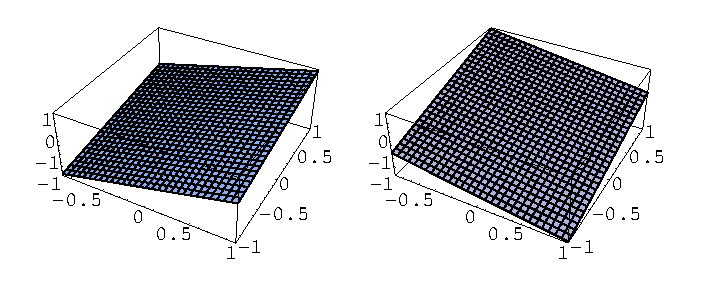
\includegraphics[width=0.7\textwidth]{fcv/analytic/velocity-stream-v0eiqz}
    \end{center}
    \caption{The velocity potential and the stream function.}
    \label{figure velocity-stream-v0eiqz}
  \end{figure}
  
  Next we find the stream lines, $\psi = c$.
  \begin{gather*}
    v_0 ( -\sin(\theta_0) x + \cos(\theta_0) y ) = c
    \\
    y = \frac{c}{v_0 \cos(\theta_0)} + \tan(\theta_0) x
  \end{gather*}
  Figure~\ref{figure streamlines-v0eiqz} shows how the streamlines go straight
  along the $\theta_0$ direction.
  \begin{figure}[htb!]
    \begin{center}
      
\includegraphics[width=0.3\textwidth]{fcv/analytic/streamlines-v0eiqz}
    \end{center}
    \caption{The streamlines.}
    \label{figure streamlines-v0eiqz}
  \end{figure}
  Next we find the velocity field.
  \begin{gather*}
    \mathbf{v} = \nabla \phi
    \\
    \mathbf{v} = \phi_x \hat{\mathbf{x}} + \phi_y \hat{\boldsymbol{y}}
    \\
    \mathbf{v} = v_0 \cos(\theta_0) \hat{\mathbf{x}} 
    + v_0 \sin(\theta_0) \hat{\boldsymbol{y}}
  \end{gather*}
  The velocity field is shown in
  Figure~\ref{figure velocity-field-v0eiqz}.
  \begin{figure}[htb!]
    \begin{center}
      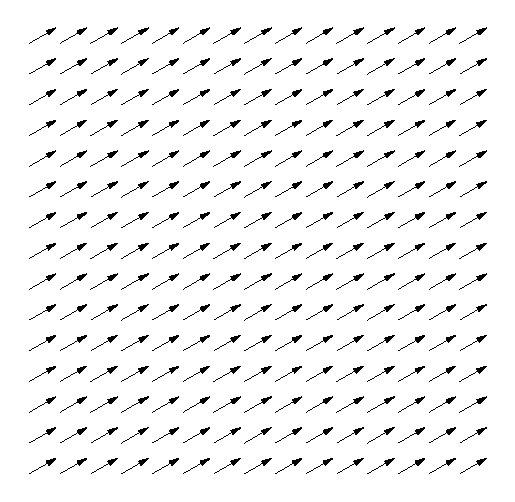
\includegraphics[width=0.4\textwidth]{fcv/analytic/velocity-field-v0eiqz}
    \end{center}
    \caption{Velocity field and velocity direction field.}
    \label{figure velocity-field-v0eiqz}
  \end{figure}
\end{Example}









\begin{Example}
  Steady, incompressible, inviscid, irrotational flow 
  is governed by the Laplace equation.  
  We consider flow around an infinite cylinder of radius $a$.  Because the
  flow does not vary along the axis of the cylinder, 
  this is a two-dimensional problem.  The flow
  corresponds to the complex potential
  \[
  \Phi(z) = v_0 \left( z + \frac{a^2}{z} \right).
  \]
  We find the velocity potential $\phi$ and stream function $\psi$.
  \begin{gather*}
    \Phi(z) = \phi + \imath \psi
    \\
    \phi = v_0 \left( r + \frac{a^2}{r} \right) \cos \theta, \quad 
    \psi = v_0 \left( r - \frac{a^2}{r} \right) \sin \theta
  \end{gather*}
  These are plotted in Figure~\ref{figure velocity-stream-v0za2z}.
  \begin{figure}[htb!]
    \begin{center}
      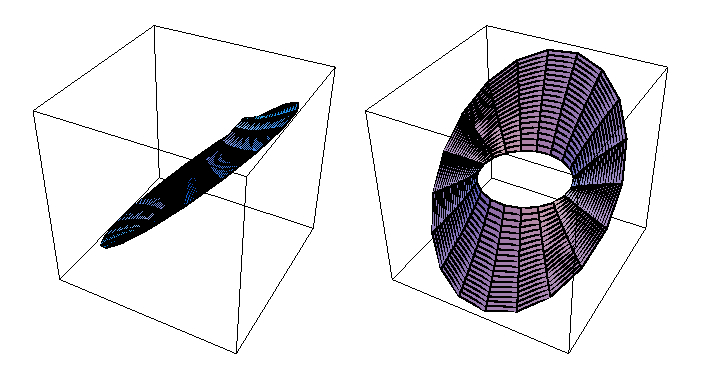
\includegraphics[width=0.8\textwidth]{fcv/analytic/velocity-stream-v0za2z}
    \end{center}
    \caption{The velocity potential and the stream function.}
    \label{figure velocity-stream-v0za2z}
  \end{figure}
  
  Next we find the stream lines, $\psi = c$.
  \begin{gather*}
    v_0 \left( r - \frac{a^2}{r} \right) \sin \theta = c
    \\
    r = \frac{ c \pm \sqrt{c^2 + 4 v_0 \sin^2 \theta} }{ 2 v_0 \sin \theta }
  \end{gather*}
  Figure~\ref{figure streamlines-v0za2z} shows how the streamlines go around
  the cylinder.
  \begin{figure}[htb!]
    \begin{center}
      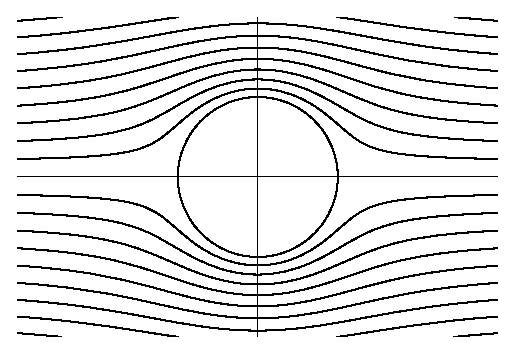
\includegraphics[width=0.4\textwidth]{fcv/analytic/streamlines-v0za2z}
    \end{center}
    \caption{The streamlines.}
    \label{figure streamlines-v0za2z}
  \end{figure}
  Next we find the velocity field.
  \begin{gather*}
    \mathbf{v} = \nabla \phi
    \\
    \mathbf{v} = \phi_r \hat{\mathbf{r}} + \frac{\phi_\theta}{r} \hat{\boldsymbol{\theta}}
    \\
    \mathbf{v} = v_0 \left(1 - \frac{a^2}{r^2} \right) \cos \theta \hat{\mathbf{r}} 
    - v_0 \left(1 + \frac{a^2}{r^2} \right) \sin \theta \hat{\boldsymbol{\theta}}
  \end{gather*}
  The velocity field is shown in
  Figure~\ref{figure velocity-field-v0za2z}.
  \begin{figure}[htb!]
    \begin{center}
      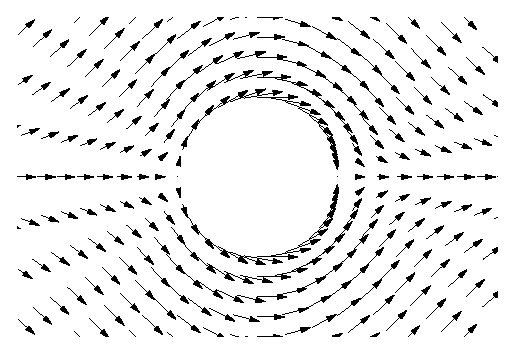
\includegraphics[width=0.5\textwidth]{fcv/analytic/velocity-field-v0za2z}
    \end{center}
    \caption{Velocity field and velocity direction field.}
    \label{figure velocity-field-v0za2z}
  \end{figure}
\end{Example}













\raggedbottom
\exercises{
%%=============================================================================
\pagebreak
\flushbottom
\section{Exercises}


%%-----------------------------------------------------------------------------
\begin{large}
  \noindent
  \textbf{Complex Derivatives}
\end{large}




\begin{Exercise}
  \label{exercise complex LHospitals rule}
  Consider two functions $f(z)$ and $g(z)$ analytic at $z_0$ with 
  $f(z_0) = g(z_0) = 0$ and $g'(z_0) \neq 0$.
  \begin{enumerate}
  \item 
    Use the definition of the complex derivative to justify L'Hospital's rule:
    \[
    \lim_{z \to z_0} \frac{f(z)}{g(z)} = \frac{f'(z_0)}{g'(z_0)}
    \]
  \item
    Evaluate the limits
    \[
    \lim_{z \to \imath} \frac{1 + z^2}{2 + 2 z^6}, \quad
    \lim_{z \to \imath \pi} \frac{\sinh(z)}{\e^z + 1}
    \]
  \end{enumerate}

  \hintsolution{complex LHospitals rule}
\end{Exercise}







%% Show that if $f(z)$ is analytic and $\phi(x,y) = f(z)$ is twice continuously
\begin{Exercise}
  \label{exercise f(z) analytic f'(z)}
  Show that if $f(z)$ is analytic and $\phi(x,y) = f(z)$ is twice continuously
  differentiable then $f'(z)$ is analytic.

  \hintsolution{f(z) analytic f'(z)}
\end{Exercise}






%% complex derivative in polar coordinates
\begin{Exercise}
  \label{exercise comp der polar}
  Find the complex derivative in the coordinate directions for 
  $f(z) = \phi(r, \theta)$.

  \hintsolution{comp der polar}
\end{Exercise}






%%
\begin{Exercise}
  \label{exercise x2y2x}
  Show that the following functions are nowhere analytic by checking where the
  derivative with respect to $z$ exists.  
  \begin{enumerate}
  \item $\sin x \cosh y - \imath \cos x \sinh y$
  \item $x^2 - y^2 + x + \imath (2 x y - y)$
  \end{enumerate}

  \hintsolution{x2y2x}
\end{Exercise}







%% $f(z_1 + z_2) = f(z_1) f(z_2)$ for all $z_1$ and $z_2$.
\begin{Exercise}
  \label{exercise f(z1+z2)=f(z1)f(z2)}
  $f(z)$ is analytic for all $z$, $(|z| < \infty)$.  
  $f\left( z_1 + z_2 \right) = f\left( z_1 \right)  f \left( z_2 \right)$ 
  for all $z_1$ and $z_2$.  (This is known
  as a \textit{functional equation}).  Prove that 
  $f(z) = \exp\left( f'(0) z \right)$.
  \index{functional equation}

  \hintsolution{f(z1+z2)=f(z1)f(z2)}
\end{Exercise}




%%-----------------------------------------------------------------------------
\begin{large}
  \noindent
  \textbf{Cauchy-Riemann Equations}
\end{large}





\begin{Exercise}
  \label{exercise constant real imaginary modulus}
  If $f(z)$ is analytic in a domain and has a constant real part,
  a constant imaginary part, or a constant modulus, show that $f(z)$ is 
  constant.

  \hintsolution{constant real imaginary modulus}
\end{Exercise}





%% e^{-z^{-4}} &\mathrm{for}\ z \neq 0, \\
\begin{Exercise}
  \label{exercise e-z-4}
  Show that the function
  \[
  f(z) = 
  \begin{cases}
    e^{-z^{-4}} &\mathrm{for}\ z \neq 0, 
    \\
    0 &\mathrm{for}\ z = 0.
  \end{cases}
  \]
  satisfies the Cauchy-Riemann equations everywhere, including at $z = 0$,
  but $f(z)$ is not analytic at the origin.

  \hintsolution{e-z-4}
\end{Exercise}





%% Cauchy-Riemann for $R(r, \theta) \e^{\imath \Theta(r,\theta)}$
\begin{Exercise}
  \label{exercise C-R polar form polar coords}
  Find the Cauchy-Riemann equations for the following forms.
  \begin{enumerate}
  \item 
    $f(z) = R(r, \theta) \e^{\imath \Theta(r,\theta)}$
  \item 
    $f(z) = R(x,y) \e^{\imath \Theta(x,y)}$
  \end{enumerate}

  \hintsolution{C-R polar form polar coords}
\end{Exercise}





%% Show that $\e^{\overline{z}}$ is not analytic.
\begin{Exercise}
  \label{exercise ol f(z)}
  \begin{enumerate}
  \item
    Show that $\e^{\overline{z}}$ is not analytic.
  \item
    $f(z)$ is an analytic function of $z$.  Show that $\overline{f}(z)
    = \overline{f\left( \overline{z} \right)}$ is also an analytic
    function of $z$.
  \end{enumerate}

  \hintsolution{ol f(z)}
\end{Exercise}








%% x^3 + y^3, \frac{x - 1}{(x-1)^2 + y^2} - \imath \frac{y}{(x-1)^2 + y^2}
\begin{Exercise}
  \label{exercise diff x3f3}
  \begin{enumerate}
  \item
    Determine all points $z = x + \imath y$ where the following functions are 
    differentiable with respect to $z$:
    \begin{enumerate}
    \item 
      $\displaystyle x^3 + y^3$
    \item 
      $\displaystyle \frac{x - 1}{(x - 1)^2 + y^2} - \imath \frac{y}{(x - 1)^2 + y^2}$
    \end{enumerate}
  \item 
    Determine all points $z$ where these functions are analytic.
  \item 
    Determine which of the following functions $v(x, y)$ are the 
    imaginary part of an analytic function $u(x, y) + \imath v(x, y)$.  For 
    those that are, compute the real part $u(x, y)$ and re-express the answer
    as an explicit function of $z = x + \imath y$:
    \begin{enumerate}
    \item 
      $x^2 - y^2$
    \item 
      $3 x^2 y$
    \end{enumerate}
  \end{enumerate}

  \hintsolution{diff x3f3}
\end{Exercise}









%% f(z) = \frac{ x^{4/3} y^{5/3} + \imath x^{5/3} y^{4/3} }{ x^2 + y^2 }
\begin{Exercise}
  \label{exercise C-R x43y53}
  Let
  \[
  f(z) = 
  \begin{cases}
    \frac{ x^{4/3} y^{5/3} + \imath x^{5/3} y^{4/3} }{ x^2 + y^2 } &\mathrm{for}\ z \neq 0, 
    \\
    0       &\mathrm{for}\ z = 0.
  \end{cases}
  \]
  Show that the Cauchy-Riemann equations hold at $z = 0$, but that $f$ is
  not differentiable at this point.

  \hintsolution{C-R x43y53}
\end{Exercise}





%% \frac{x^3(1+\imath)-y^3(1-\imath)}{x^2+y^2} &\mathrm{for}\ z \neq 0, \\
\begin{Exercise}
  \label{exercise C-R x31iy31i}
  Consider the complex function 
  \[
  f(z) = u + \imath v = 
  \begin{cases}
    \frac{x^3 (1 + \imath) - y^3 (1 - \imath)}{x^2 + y^2} &\mathrm{for}\ z \neq 0, 
    \\
    0 &\mathrm{for}\ z= 0.
  \end{cases}
  \]
  Show that the partial derivatives of $u$ and $v$ with respect to $x$
  and $y$ exist at $z = 0$ and that $u_x = v_y$ and $u_y = -v_x$ there: the
  Cauchy-Riemann equations are satisfied at $z = 0$. On the other hand,
  show that
  \[
  \lim_{z \to 0} \frac{f(z)}{z}
  \]
  does not exist, that is, $f$ is not complex-differentiable at $z = 0$.

  \hintsolution{C-R x31iy31i}
\end{Exercise}








%% Show that the logarithm $\log z$ is differentiable for $z \neq 0$.
\begin{Exercise}
  \label{exercise diff log}
  Show that the logarithm $\log z$ is differentiable for $z \neq 0$.
  Find the derivative of the logarithm.

  \hintsolution{diff log}
\end{Exercise}









%% \frac{\dd f}{\dd z} = \e^{- \imath \theta} \frac{\partial f}{\partial r}
\begin{Exercise}
  \label{exercise diff polar coords}
  Show that the Cauchy-Riemann equations for the analytic function 
  $f(z) = u(r, \theta) + \imath v(r, \theta)$ are
  \[
  u_r = v_\theta / r, \quad u_\theta = - r v_r.
  \]

  \hintsolution{diff polar coords}
\end{Exercise}









%% $w = u + \imath v$ is an analytic function of $z$. 
\begin{Exercise}
  \label{exercise w=u+iv is analytic}
  $w = u + \imath v$ is an analytic function of $z$.  $\phi(x, y)$ is an
  arbitrary smooth function of $x$ and $y$.  When expressed in terms of 
  $u$ and $v$, $\phi(x, y) = \Phi(u, v)$.  Show that ($w' \neq 0$)
  \[
  \frac{\partial \Phi}{\partial u} - \imath  \frac{\partial \Phi}{\partial v} = 
  \left( \frac{\dd w}{\dd z} \right)^{-1} 
  \left( \frac{\partial \phi}{\partial x} - \imath  \frac{\partial \phi}{\partial y} \right).
  \]
  Deduce
  \[
  \frac{\partial^2 \Phi}{\partial u^2} + \frac{\partial^2 \Phi}{\partial v^2} =
  \left| \frac{\dd w}{\dd z} \right|^{-2} 
  \left( \frac{\partial^2 \phi}{\partial x^2} + \frac{\partial^2 \phi}{\partial y^2} \right).
  \]

  \hintsolution{w=u+iv is analytic}
\end{Exercise}




%% log and square root are analytic
\begin{Exercise}
  \label{exercise log square root}
  Show that the functions defined by $f(z) =
  \log|z| + \imath  \arg(z)$ and $f(z) = \sqrt{|z|} \e^{\imath \arg(z)/2}$ are
  analytic in the sector $|z| > 0$, $|\arg(z)| < \pi$. What
  are the corresponding derivatives $\dd f / \dd z$?

  \hintsolution{log square root}
\end{Exercise}







%% $u(x,y) = x \Log(r) -y \arctan(x, y)$ ($r\neq 0$)
\begin{Exercise}
  \label{exercise xlogr yarctanxy}
  Show that the following functions are harmonic.
  For each one of them find its harmonic conjugate and form the
  corresponding holomorphic function.  
  \begin{enumerate}
  \item
    $u(x,y) = x \Log(r) - y \arctan(x, y)$ ($r \neq 0$)
  \item
    $u(x,y) = \arg(z)$ ($|\arg(z)| < \pi$, $r \neq 0$)
  \item
    $u(x,y) = r^n \cos(n \theta)$
  \item
    $u(x,y) = y/r^2$ ($r \neq 0$)
  \end{enumerate}

  \hintsolution{xlogr yarctanxy}
\end{Exercise}






\begin{Exercise}
  \label{exercise cr xy2 i2xy}
  \begin{enumerate}
  \item 
    Use the Cauchy-Riemann equations to determine where the function
    \[
    f(z) = (x - y)^2 + \imath 2 (x + y)
    \]
    is differentiable and where it is analytic.
  \item 
    Evaluate the derivative of
    \[
    f(z) = \e^{x^2 - y^2} ( \cos(2 x y) + \imath \sin(2 x y) )
    \]
    and describe the domain of analyticity.
  \end{enumerate}

  \hintsolution{cr xy2 i2xy}
\end{Exercise}






\begin{Exercise}
  \label{exercise cartesian cr polar cr}
  Consider the function $f(z) = u + \imath v$ with real and imaginary parts
  expressed in terms of either $x$ and $y$ or $r$ and $\theta$.
  \begin{enumerate}
  \item 
    Show that the Cauchy-Riemann equations
    \[
    u_x = v_y, \quad u_y = - v_x
    \]
    are satisfied and these partial derivatives are continuous at a point $z$ 
    if and only if the polar form of the Cauchy-Riemann equations
    \[
    u_r = \frac{1}{r} v_\theta, \quad \frac{1}{r} u_\theta = - v_r
    \]
    is satisfied and these partial derivatives are continuous there.
  \item 
    Show that it is easy to verify that $\Log z$ is analytic for $r > 0$
    and $- \pi < \theta < \pi$
    using the polar form of the Cauchy-Riemann equations and that the value
    of the derivative is easily obtained from a polar differentiation formula.
  \item 
    Show that in polar coordinates, Laplace's equation becomes
    \[
    \phi_{r r} + \frac{1}{r} \phi_r + \frac{1}{r^2} \phi_{\theta \theta} = 0.
    \]
  \end{enumerate}

  \hintsolution{cartesian cr polar cr}
\end{Exercise}







\begin{Exercise}
  \label{exercise real part x3 y3}
  Determine which of the following functions are the real parts of an analytic
  function.
  \begin{enumerate}
  \item 
    $u(x,y) = x^3 - y^3$
  \item 
    $u(x,y) = \sinh x \cos y + x$
  \item
    $u(r,\theta) = r^n \cos(n \theta)$
  \end{enumerate}
  and find $f(z)$ for those that are.

  \hintsolution{real part x3 y3}
\end{Exercise}





\begin{Exercise}
  \label{exercise potential flow log z-1 log z+1}
  Consider steady, incompressible, inviscid, irrotational flow governed by the
  Laplace equation.  Determine the form of the velocity potential and stream
  function contours for the complex potentials
  \begin{enumerate}
  \item $\Phi(z) = \phi(x,y) + \imath \psi(x,y) = \log z + \imath \log z$
  \item $\Phi(z) = \log(z - 1) + \log(z + 1)$
  \end{enumerate}
  Plot and describe the features of the flows you are considering.

  \hintsolution{potential flow log z-1 log z+1}
\end{Exercise}



\begin{Exercise}
  \label{exercise classify z z2+1}
\begin{enumerate}
\item 
  Classify all the singularities (removable, poles, isolated essential,
  branch points, non-isolated essential) of the following 
  functions in the extended complex plane
  \begin{enumerate}
  \item 
    $\displaystyle \frac{z}{z^2 + 1}$
  \item 
    $\displaystyle \frac{1}{\sin z}$
  \item 
    $\displaystyle \log \left( 1 + z^2 \right)$
  \item 
    $\displaystyle z \sin(1/z)$
  \item 
    $\displaystyle \frac{ \tan^{-1}(z)}{z \sinh^2(\pi z)}$
  \end{enumerate}
\item 
  Construct functions that have the following zeros or singularities:
  \begin{enumerate}
  \item 
    a simple zero at $z = \imath$ and an isolated essential singularity at $z = 1$.
  \item 
    a removable singularity at $z = 3$, a pole of order 6 at $z = - \imath$ 
    and an essential singularity at $z_\infty$.
  \end{enumerate}
\end{enumerate}

  \hintsolution{classify z z2+1}
\end{Exercise}










\raggedbottom
}
%%=============================================================================
\hints{
\pagebreak
\flushbottom
\section{Hints}





%%-----------------------------------------------------------------------------
\begin{large}
  \noindent
  \textbf{Complex Derivatives}
\end{large}





\begin{Hint}
  \label{hint complex LHospitals rule}
\end{Hint}






%% Show that if $f(z)$ is analytic and $\phi(x,y) = f(z)$ is twice continuously
\begin{Hint}
  \label{hint f(z) analytic f'(z)}
  Start with the Cauchy-Riemann equation and then differentiate with respect
  to $x$.
\end{Hint}




%% complex derivative in polar coordinates
\begin{Hint}
  \label{hint comp der polar}
  Read Example~\ref{complex_deriv_cart} and use
  Result~\ref{result complex derivative}.
\end{Hint}





%%
\begin{Hint}
  \label{hint x2y2x}
  Use Result~\ref{result complex derivative}.
\end{Hint}






%% $f(z_1 + z_2) = f(z_1) f(z_2)$ for all $z_1$ and $z_2$.
\begin{Hint}
  \label{hint f(z1+z2)=f(z1)f(z2)}
  Take the logarithm of the equation to get a linear equation.
\end{Hint}





%%-----------------------------------------------------------------------------
\begin{large}
  \noindent
  \textbf{Cauchy-Riemann Equations}
\end{large}




\begin{Hint}
  \label{hint constant real imaginary modulus}
\end{Hint}





%% e^{-z^{-4}} &\mathrm{for}\ z \neq 0, \\
\begin{Hint}
  \label{hint e-z-4}
\end{Hint}




%% Cauchy-Riemann for $R(r, \theta) \e^{\imath \Theta(r,\theta)}$
\begin{Hint}
  \label{hint C-R polar form polar coords}
  For the first part use the result of Exercise~\ref{exercise comp der polar}.
\end{Hint}





%% Show that $\e^{\overline{z}}$ is not analytic.
\begin{Hint}
  \label{hint ol f(z)}
  Use the Cauchy-Riemann equations.
\end{Hint}







%% x^3 + y^3, \frac{x - 1}{(x-1)^2 + y^2} - \imath \frac{y}{(x-1)^2 + y^2}
\begin{Hint}
  \label{hint diff x3f3}
  %% CONTINUE
\end{Hint}











%% f(z) = \frac{ x^{4/3} y^{5/3} + \imath x^{5/3} y^{4/3} }{ x^2 + y^2 }
\begin{Hint}
  \label{hint C-R x43y53}
  To evaluate $u_x(0,0)$, etc. use the definition of differentiation.
  Try to find $f'(z)$ with the definition of complex differentiation.
  Consider $\Delta z = \Delta r \e^{\imath \theta}$.
\end{Hint}





%% \frac{x^3(1+\imath)-y^3(1-\imath)}{x^2+y^2} &\mathrm{for}\ z \neq 0, \\
\begin{Hint}
  \label{hint C-R x31iy31i}
  To evaluate $u_x(0,0)$, etc. use the definition of differentiation.
  Try to find $f'(z)$ with the definition of complex differentiation.
  Consider $\Delta z = \Delta r \e^{\imath \theta}$.
\end{Hint}







%% Show that the logarithm $\log z$ is differentiable for $z \neq 0$.
\begin{Hint}
  \label{hint diff log}
  %% CONTINUE
\end{Hint}




%% \frac{\dd f}{\dd z} = \e^{- \imath \theta} \frac{\partial f}{\partial r}
\begin{Hint}
  \label{hint diff polar coords}
  %% CONTINUE
\end{Hint}







%% $w = u + \imath v$ is an analytic function of $z$. 
\begin{Hint}
  \label{hint w=u+iv is analytic}
  %% CONTINUE
\end{Hint}





%% log and square root are analytic
\begin{Hint}
  \label{hint log square root}
\end{Hint}






%% $u(x,y) = x \Log(r) -y \arctan(x, y)$ ($r\neq 0$)
\begin{Hint}
  \label{hint xlogr yarctanxy}
\end{Hint}






\begin{Hint}
  \label{hint cr xy2 i2xy}
\end{Hint}





\begin{Hint}
  \label{hint cartesian cr polar cr}
\end{Hint}







\begin{Hint}
  \label{hint real part x3 y3}
\end{Hint}







\begin{Hint}
  \label{hint potential flow log z-1 log z+1}
\end{Hint}



\begin{Hint}
  \label{hint classify z z2+1}
  %%CONTINUE
\end{Hint}



\raggedbottom
}
%%=============================================================================
\solutions{
\pagebreak
\flushbottom
\section{Solutions}







%%-----------------------------------------------------------------------------
\begin{large}
  \noindent
  \textbf{Complex Derivatives}
\end{large}






\begin{Solution}
  \label{solution complex LHospitals rule}
  \begin{enumerate}
  \item 
    We consider L'Hospital's rule.
    \[
    \lim_{z \to z_0} \frac{f(z)}{g(z)} = \frac{f'(z_0)}{g'(z_0)}
    \]
    We start with the right side and show that it is equal to the left side.
    First we apply the definition of complex differentiation.
    \[
    \frac{f'(z_0)}{g'(z_0)} 
    = \frac{ \lim_{\epsilon \to 0} \frac{f(z_0 + \epsilon) - f(z_0)}{\epsilon} }
    { \lim_{\delta \to 0} \frac{g(z_0 + \delta) - g(z_0)}{\delta} }
    = \frac{ \lim_{\epsilon \to 0} \frac{f(z_0 + \epsilon)}{\epsilon} }
    { \lim_{\delta \to 0} \frac{g(z_0 + \delta)}{\delta} }
    \]
    Since both of the limits exist, we may take the limits with $\epsilon = \delta$.
    \begin{gather*}
      \frac{f'(z_0)}{g'(z_0)} = \lim_{\epsilon \to 0} \frac{ f(z_0 + \epsilon) }{ g(z_0 + \epsilon) }
      \\
      \frac{f'(z_0)}{g'(z_0)} = \lim_{z \to z_0} \frac{ f(z) }{ g(z) }
    \end{gather*}
    This proves L'Hospital's rule.
  \item
    \[
    \lim_{z \to \imath} \frac{1 + z^2}{2 + 2 z^6}
    = \left[ \frac{2 z}{12 z^5} \right]_{z = \imath}
    = \frac{1}{6}
    \]
    \begin{align*}
      \lim_{z \to \imath \pi} \frac{\sinh(z)}{\e^z + 1}
      = \left[ \frac{\cosh(z)}{\e^z} \right]_{z = \imath \pi}
      = 1
    \end{align*}
  \end{enumerate}
\end{Solution}












%% Show that if $f(z)$ is analytic and $\phi(x,y) = f(z)$ is twice continuously
\begin{Solution}
  \label{solution f(z) analytic f'(z)}
  We start with the Cauchy-Riemann equation and then differentiate 
  with respect to $x$.
  \begin{gather*}
    \phi_x = - \imath \phi_y 
    \\
    \phi_{x x} = - \imath \phi_{y x}
  \end{gather*}
  We interchange the order of differentiation.
  \begin{gather*}
    \left( \phi_x \right)_x = - \imath  \left( \phi_x \right)_y 
    \\
    \left( f' \right)_x = - \imath  \left( f' \right)_y
  \end{gather*}
  Since $f'(z)$ satisfies the Cauchy-Riemann equation and its 
  partial derivatives exist and are continuous, it is analytic.
\end{Solution}






%% complex derivative in polar coordinates
\begin{Solution}
  \label{solution comp der polar}
  We calculate the complex derivative in the coordinate directions.
  \begin{gather*}
    \frac{\dd f}{\dd z} 
    = \left( \frac{\partial \left( r \e^{\imath \theta} \right)}{\partial r} \right)^{-1}  
    \frac{\partial \phi}{\partial r} = \e^{ -\imath \theta } \frac{\partial \phi}{\partial r}, 
    \\
    \frac{\dd f}{\dd z} 
    = \left( \frac{\partial \left( r \e^{\imath \theta} \right)}{\partial \theta} \right)^{-1} 
    \frac{\partial \phi}{\partial \theta} = - \frac{\imath}{r} \e^{-\imath \theta} \frac{\partial \phi}{\partial \theta}.
  \end{gather*}
  We can write this in operator notation.
  \[
  \frac{\dd}{\dd z} = \e^{-\imath \theta} \frac{\partial}{\partial r} 
  = - \frac{\imath}{r} \e^{-\imath \theta} \frac{\partial}{\partial \theta}
  \]
\end{Solution}












%%
\begin{Solution}
  \label{solution x2y2x}
  \begin{enumerate}
    %%- - - - - - - - - - - - - - - - - - - - - - - - - - - - - - - - - - -
  \item
    Consider $f(x,y) = \sin x \cosh y - \imath \cos x \sinh y$.
    The derivatives in the $x$ and $y$ directions are
    \begin{align*}
      \frac{\partial f}{\partial x} &= \cos x \cosh y + \imath \sin x \sinh y 
      \\
      -\imath  \frac{\partial f}{\partial y} &= - \cos x \cosh y - \imath \sin x \sinh y
    \end{align*}
    These derivatives exist and are everywhere continuous.  We equate the
    expressions to get a set of two equations.
    \begin{gather*}
      \cos x \cosh y = - \cos x \cosh y, \qquad
      \sin x \sinh y = - \sin x \sinh y 
      \\
      \cos x \cosh y = 0, \qquad
      \sin x \sinh y = 0 
      \\
      \left( x = \frac{\pi}{2} + n \pi \right)\ \mathrm{and}\ 
      \left( x = m \pi\ \mathrm{or}\ y = 0 \right) 
    \end{gather*}
    The function may be differentiable only at the points
    \[
    \boxed{
      x = \frac{\pi}{2} + n \pi, \quad y = 0.
      }
    \]
    Thus the function is nowhere analytic.
    %%- - - - - - - - - - - - - - - - - - - - - - - - - - - - - - - - - - -
  \item 
    Consider $f(x,y) = x^2 - y^2 + x + \imath (2 x y - y)$.
    The derivatives in the $x$ and $y$ directions are
    \begin{align*}
      \frac{\partial f}{\partial x} &= 2 x + 1 + \imath 2 y 
      \\
      -\imath  \frac{\partial f}{\partial y} &= \imath 2 y + 2 x - 1
    \end{align*}
    These derivatives exist and are everywhere continuous.  We equate the
    expressions to get a set of two equations.
    \[
    2 x + 1 = 2 x - 1, \qquad 2 y = 2 y.
    \]
    Since this set of equations has no solutions, there are no points at which
    the function is differentiable.  The function is nowhere analytic.
  \end{enumerate}
\end{Solution}







%% $f(z_1 + z_2) = f(z_1) f(z_2)$ for all $z_1$ and $z_2$.
\begin{Solution}
  \label{solution f(z1+z2)=f(z1)f(z2)}
  \begin{gather*}
    f\left( z_1 + z_2 \right) = f\left( z_1 \right) f\left( z_2 \right) 
    \\
    \log\left( f\left( z_1 + z_2 \right) \right) 
    = \log\left( f\left( z_1 \right) \right) 
    + \log\left( f\left( z_2 \right) \right) 
    \\
    \intertext{We define $g(z) = \log( f(z) )$.}
    g\left( z_1 + z_2 \right) = g\left( z_1 \right) + g\left( z_2 \right) 
    \\
    \intertext{This is a linear equation which has exactly the solutions:}
    g(z) = c z.
  \end{gather*}
  Thus $f(z)$ has the solutions:
  \[
  f(z) = \e^{c z},
  \]
  where $c$ is any complex constant.  We can write this constant in terms 
  of $f'(0)$.   We differentiate the original equation with respect to $z_1$
  and then substitute $z_1 = 0$.
  \begin{gather*}
    f'\left( z_1 + z_2 \right) = f'\left( z_1 \right) f\left( z_2 \right) 
    \\
    f'\left( z_2 \right) = f'(0) f\left( z_2 \right) 
    \\
    f'(z) = f'(0) f(z) 
    \\
    \intertext{We substitute in the form of the solution.}
    c \e^{c z} = f'(0) \e^{c z} 
    \\
    c = f'(0)
  \end{gather*}
  Thus we see that
  \[
  f(z) = \e^{f'(0) z}.
  \]
\end{Solution}




%%-----------------------------------------------------------------------------
\begin{large}
  \noindent
  \textbf{Cauchy-Riemann Equations}
\end{large}





\begin{Solution}
  \label{solution constant real imaginary modulus}
  \textbf{Constant Real Part.}
  First assume that $f(z)$ has constant real part.  We solve the 
  Cauchy-Riemann equations to determine the imaginary part.
  \begin{gather*}
    u_x = v_y, \quad u_y = - v_x
    \\
    v_x = 0, \quad v_y = 0
  \end{gather*}
  We integrate the first equation to obtain $v = a + g(y)$ where $a$ is a 
  constant and $g(y)$ is an arbitrary function.  Then we substitute this 
  into the second equation to determine $g(y)$.
  \begin{gather*}
    g'(y) = 0
    \\
    g(y) = b
  \end{gather*}
  We see that the imaginary part of $f(z)$ is a constant and conclude 
  that $f(z)$ is constant.


  \textbf{Constant Imaginary Part.}
  Next assume that $f(z)$ has constant imaginary part.  We solve the 
  Cauchy-Riemann equations to determine the real part.
  \begin{gather*}
    u_x = v_y, \quad u_y = - v_x
    \\
    u_x = 0, \quad u_y = 0
  \end{gather*}
  We integrate the first equation to obtain $u = a + g(y)$ where $a$ is a 
  constant and $g(y)$ is an arbitrary function.  Then we substitute this 
  into the second equation to determine $g(y)$.
  \begin{gather*}
    g'(y) = 0
    \\
    g(y) = b
  \end{gather*}
  We see that the real part of $f(z)$ is a constant and conclude 
  that $f(z)$ is constant.


  \textbf{Constant Modulus.}
  Finally assume that $f(z)$ has constant modulus.  
  \begin{gather*}
    |f(z)| = \mathrm{constant}
    \\
    \sqrt{u^2 + v^2} = \mathrm{constant}
    \\
    u^2 + v^2 = \mathrm{constant}
  \end{gather*}
  We differentiate this equation with respect to $x$ and $y$.
  \begin{gather*}
    2 u u_x + 2 v v_x = 0, \quad 2 u u_y + 2 v v_y = 0
    \\  
    \begin{pmatrix}
      u_x & v_x \\
      u_y & v_y
    \end{pmatrix}
    \begin{pmatrix}
      u \\
      v
    \end{pmatrix}
    = 0
  \end{gather*}
  This system has non-trivial solutions for $u$ and $v$ only if the matrix
  is non-singular.  (The trivial solution $u = v = 0$ is the constant function
  $f(z) = 0$.)  We set the determinant of the matrix to zero.
  \[
  u_x v_y - u_y v_x = 0
  \]
  We use the Cauchy-Riemann equations to write this in terms of $u_x$ and $u_y$.
  \begin{gather*}
    u_x^2 + u_y^2 = 0
    \\
    u_x = u_y = 0
  \end{gather*}
  Since its partial derivatives vanish, $u$ is a constant.  
  From the Cauchy-Riemann equations we see
  that the partial derivatives of $v$ vanish as well, so it is constant.
  We conclude that $f(z)$ is a constant.


  \textbf{Constant Modulus.}
  Here is another method for the constant modulus case.
  We solve the Cauchy-Riemann equations in polar form to determine the 
  argument of $f(z) = R(x,y) \e^{\imath \Theta(x,y)}$.  Since the function has constant
  modulus $R$, its partial derivatives vanish.
  \begin{gather*}
    R_x = R \Theta_y, \quad R_y = - R \Theta_x
    \\
    R \Theta_y = 0, \quad R \Theta_x = 0
  \end{gather*}
  The equations are satisfied for $R = 0$.  For this case, $f(z) = 0$. 
  We consider nonzero $R$.
  \[
  \Theta_y = 0, \quad \Theta_x = 0
  \]
  We see that the argument of $f(z)$ is a constant and conclude 
  that $f(z)$ is constant.
\end{Solution}






%% e^{-z^{-4}} &\mathrm{for}\ z \neq 0, \\
\begin{Solution}
  \label{solution e-z-4}
  First we verify that the Cauchy-Riemann equations are satisfied for 
  $z \neq 0$.  Note that the form
  \[
  f_x = - \imath f_y
  \]
  will be far more convenient than the form
  \[
  u_x = v_y, \quad u_y = - v_x
  \]
  for this problem.
  \begin{gather*}
    f_x = 4 (x + \imath y)^{-5} \e^{-(x + \imath y)^{-4}} 
    \\
    -\imath f_y = -\imath 4 (x + \imath y)^{-5} \imath  \e^{-(x + \imath y)^{-4}} 
    = 4 (x + \imath y)^{-5} \e^{-(x + \imath y)^{-4}}
  \end{gather*}
  The Cauchy-Riemann equations are satisfied for $z \neq 0$.

  Now we consider the point $z = 0$.
  \begin{align*}
    f_x(0,0) &= \lim_{\Delta x \to 0} \frac{f(\Delta x, 0) - f(0,0)}{ \Delta x } 
    \\
    &= \lim_{\Delta x \to 0} \frac{\e^{-\Delta x^{-4}} }{ \Delta x } 
    \\
    &= 0
  \end{align*}
  \begin{align*}
    -\imath f_y(0,0) &= -\imath \lim_{\Delta y \to 0} \frac{f(0, \Delta y) - f(0,0)}{ \Delta y } 
    \\
    &= -\imath \lim_{\Delta y \to 0} \frac{\e^{-\Delta y^{-4}} }{ \Delta y } 
    \\
    &= 0
  \end{align*}
  The Cauchy-Riemann equations are satisfied for $z = 0$.



  $f(z)$ is not analytic at the point $z = 0$.  We show this by calculating
  the derivative.
  \[
  f'(0) = \lim_{\Delta z \to 0} \frac{f(\Delta z) - f(0)}{\Delta z}
  = \lim_{\Delta z \to 0} \frac{f(\Delta z)}{\Delta z}
  \]
  Let $\Delta z = \Delta r \e^{\imath \theta}$, that is, we approach the origin
  at an angle of $\theta$.
  \begin{align*}
    f'(0)   &= \lim_{\Delta r \to 0} \frac{ f\left( \Delta r \e^{\imath \theta} \right)}{\Delta r \e^{\imath \theta} } 
    \\
    &= \lim_{\Delta r \to 0} \frac{ \e^{- r^{-4} \e^{-\imath 4 \theta} } }{ \Delta r \e^{\imath \theta} }
  \end{align*}
  For most values of $\theta$ the limit does not exist.  Consider $\theta = \pi / 4$.
  \[
  f'(0) = \lim_{\Delta r \to 0} \frac{ \e^{r^{-4} } }{ \Delta r \e^{\imath \pi / 4} } = \infty
  \]
  Because the limit does not exist,  the function is 
  not differentiable at $z = 0$.  Recall that satisfying the Cauchy-Riemann 
  equations is a necessary, but not a sufficient condition for 
  differentiability.  
\end{Solution}





%% Cauchy-Riemann for $R(r, \theta) \e^{\imath \Theta(r,\theta)}$
\begin{Solution}
  \label{solution C-R polar form polar coords}
  \begin{enumerate}
  \item 
    We find the Cauchy-Riemann equations for 
    \[
    f(z) = R(r, \theta) \e^{\imath \Theta(r,\theta)}.
    \]
    From Exercise~\ref{exercise comp der polar} we know that the complex 
    derivative in the polar coordinate directions is
    \[
    \frac{\dd}{\dd z} = \e^{-\imath \theta} \frac{\partial}{\partial r} 
    = - \frac{\imath}{r} \e^{-\imath \theta} \frac{\partial}{\partial \theta}.
    \]
    We equate the derivatives in the two directions.
    \begin{gather*}
      \e^{-\imath \theta} \frac{\partial}{\partial r} \left[ R \e^{\imath \Theta} \right] 
      = - \frac{\imath}{r} \e^{-\imath \theta} \frac{\partial}{\partial \theta} \left[ R \e^{\imath \Theta} \right] 
      \\
      \left( R_r + \imath R \Theta_r \right) \e^{\imath \Theta} 
      = - \frac{\imath}{r} \left( R_\theta + \imath R \Theta_\theta \right) \e^{\imath \Theta}
    \end{gather*}
    We divide by $\e^{\imath \Theta}$ and equate the real and imaginary components
    to obtain the Cauchy-Riemann equations.
    \[
    R_r = \frac{R}{r} \Theta_\theta, \qquad
    \frac{1}{r} R_\theta = - R \Theta_r
    \]
  \item
    We find the Cauchy-Riemann equations for 
    \[
    f(z) = R(x,y) \e^{\imath \Theta(x,y)}.
    \]
    We equate the derivatives in the $x$ and $y$ directions.
    \begin{gather*}
      \frac{\partial}{\partial x} \left[ R \e^{\imath \Theta} \right] 
      = - \imath  \frac{\partial}{\partial y} \left[ R \e^{\imath \Theta} \right] 
      \\
      \left( R_x + \imath R \Theta_y \right) \e^{\imath \Theta} 
      = - \imath  \left( R_x + \imath R \Theta_y \right) \e^{\imath \Theta}
    \end{gather*}
    We divide by $\e^{\imath \Theta}$ and equate the real and imaginary components
    to obtain the Cauchy-Riemann equations.
    \[
    R_x = R \Theta_y, \qquad
    R_y = - R \Theta_x
    \]
  \end{enumerate}
\end{Solution}






%% Show that $\e^{\overline{z}}$ is not analytic.
\begin{Solution}
  \label{solution ol f(z)}
  \begin{enumerate}
    %%
    %%
    %%
  \item
    A necessary condition for analyticity in an open set is that the 
    Cauchy-Riemann equations are satisfied in that set.  
    We write $\e^{\overline{z}}$ in Cartesian form.
    \[
    \e^{\overline{z}} = \e^{x - \imath y} = \e^x \cos y - \imath  \e^x \sin y.
    \]
    Now we determine where $u = \e^x \cos y$ and $v = - \e^x \sin y$ satisfy the
    Cauchy-Riemann equations.
    \begin{gather*}
      u_x = v_y,
      \qquad
      u_y = - v_x 
      \\
      \e^x \cos y = - \e^x \cos y,
      \qquad
      - \e^x \sin y = \e^x \sin y 
      \\
      \cos y = 0,
      \qquad
      \sin y = 0 \\
      y = \frac{\pi}{2} + \pi m,
      \qquad
      y = \pi n
    \end{gather*}
    Thus we see that the Cauchy-Riemann equations are not satisfied anywhere.
    $\e^{\overline{z}}$ is nowhere analytic.
    %%
    %%
    %%
  \item
    Since $f(z) = u + \imath v$ is analytic, $u$ and $v$ satisfy the 
    Cauchy-Riemann equations and their first partial derivatives 
    are continuous.
    \[
    \overline{f}(z) = \overline{f\left( \overline{z} \right)} 
    = \overline{u(x, -y) + \imath v(x, -y)}
    = u(x, -y) - \imath v(x, -y)
    \]
    We define $\overline{f}(z) \equiv \mu(x, y) + \imath \nu(x, y) = u(x, -y) - \imath v(x, y)$.
    Now we see if $\mu$ and $\nu$ satisfy the Cauchy-Riemann equations.
    \begin{gather*}
      \mu_x = \nu_y, \qquad \mu_y = - \nu_x 
      \\
      (u(x, -y))_x = (-v(x, -y))_y, \qquad 
      (u(x, -y))_y = - (-v(x, -y))_x 
      \\
      u_x(x, -y) = v_y(x, -y), \qquad
      - u_y(x, -y) = v_x(x, -y) 
      \\
      u_x = v_y, \qquad u_y = - v_x 
    \end{gather*}
    Thus we see that the Cauchy-Riemann equations for $\mu$ and $\nu$ are
    satisfied if and only if the Cauchy-Riemann equations for $u$ and $v$
    are satisfied.  The continuity of the first partial derivatives of 
    $u$ and $v$ implies the same of $\mu$ and $\nu$.  Thus 
    $\overline{f}(z)$ is analytic.
  \end{enumerate}
\end{Solution}







%% x^3 + y^3, \frac{x - 1}{(x-1)^2 + y^2} - \imath \frac{y}{(x-1)^2 + y^2}
\begin{Solution}
  \label{solution diff x3f3}
  \begin{enumerate}
    %%
    %%
  \item
    The necessary condition for a function $f(z) = u + \imath v$ to be
    differentiable at a point is that the Cauchy-Riemann equations
    hold and the first partial derivatives of $u$ and $v$ are
    continuous at that point.
    \begin{enumerate}
      %%
    \item
      \[
      f(z) = x^3 + y^3 + \imath 0
      \]
      The Cauchy-Riemann equations are
      \begin{gather*}
        u_x = v_y \quad \mathrm{and} \quad u_y = - v_x 
        \\
        3 x^2 = 0 \quad \mathrm{and} \quad 3 y^2 = 0 
        \\
        x = 0 \quad \mathrm{and} \quad y = 0 
      \end{gather*}
      The first partial derivatives are continuous.  Thus we see that the 
      function is differentiable only at the point $z = 0$.
      %%
    \item
      \[
      f(z) = \frac{x - 1}{(x - 1)^2 + y^2} - \imath  \frac{y}{(x - 1)^2 + y^2}
      \]
      The Cauchy-Riemann equations are
      \begin{gather*}
        u_x = v_y \quad \mathrm{and} \quad u_y = - v_x 
        \\
        \frac{-(x - 1)^2 + y^2}{((x - 1)^2 + y^2)^2} 
        = \frac{-(x - 1)^2 + y^2}{((x - 1)^2 + y^2)^2} 
        \quad \mathrm{and} \quad 
        \frac{2 (x - 1) y}{((x - 1)^2 + y^2)^2} 
        = \frac{2 (x - 1) y}{((x - 1)^2 + y^2)^2} 
      \end{gather*}
      The Cauchy-Riemann equations are each identities.  The first
      partial derivatives are continuous everywhere except the point
      $x = 1$, $y = 0$.  Thus the function is differentiable
      everywhere except $z = 1$.
    \end{enumerate}
    %%
    %%
  \item
    \begin{enumerate}
      %%
    \item
      The function is not differentiable in any open set.  Thus the 
      function is nowhere analytic.
      %%
    \item
      The function is differentiable everywhere except $z = 1$.  Thus 
      the function is analytic everywhere except $z = 1$.
    \end{enumerate}
    %%
    %%
  \item
    \begin{enumerate}
      %%
    \item
      First we determine if the function is harmonic.
      \begin{gather*}
        v = x^2 - y^2 
        \\
        v_{x x} + v_{y y} = 0 
        \\
        2 - 2 = 0
      \end{gather*}
      The function is harmonic in the complex plane and this is the
      imaginary part of some analytic function.  By inspection, we see
      that this function is
      \[
      \imath z^2 + c = - 2 x y + c + \imath  \left( x^2 - y^2 \right),
      \]
      where $c$ is a real constant.
      We can also find the function by solving the Cauchy-Riemann equations.
      \begin{gather*}
        u_x = v_y \quad \mathrm{and} \quad u_y = - v_x 
        \\
        u_x = - 2 y \quad \mathrm{and} \quad u_y = - 2 x 
        \\
        \intertext{We integrate the first equation.}
        u = - 2 x y + g(y) 
        \\
        \intertext{Here $g(y)$ is a function of integration.  We substitute 
          this into the second Cauchy-Riemann equation to determine $g(y)$.}
        u_y = - 2 x 
        \\
        -2 x + g'(y) = -2 x 
        \\
        g'(y) = 0 
        \\
        g(y) = c 
        \\
        u = - 2 x y + c 
        \\
        f(z) = -2 x y + c + \imath  \left( x^2 - y^2 \right) 
        \\
        f(z) = \imath z^2 + c
      \end{gather*}
      %%
    \item
      First we determine if the function is harmonic.
      \begin{gather*}
        v = 3 x^2 y 
        \\
        v_{x x} + v_{y y} = 6 y 
      \end{gather*}
      The function is not harmonic.  It is not the imaginary 
      part of some analytic function.  
    \end{enumerate}
  \end{enumerate}
\end{Solution}











%% f(z) = \frac{ x^{4/3} y^{5/3} + \imath x^{5/3} y^{4/3} }{ x^2 + y^2 }
\begin{Solution}
  \label{solution C-R x43y53}
  We write the real and imaginary parts of $f(z) = u + \imath v$.
  \[
  u = 
  \begin{cases}
    \frac{ x^{4/3} y^{5/3} }{ x^2 + y^2 } &\mathrm{for}\ z \neq 0, 
    \\
    0       &\mathrm{for}\ z = 0.
  \end{cases}, \qquad
  v = 
  \begin{cases}
    \frac{ x^{5/3} y^{4/3} }{ x^2 + y^2 } &\mathrm{for}\ z \neq 0, 
    \\
    0       &\mathrm{for}\ z = 0.
  \end{cases}
  \]
  The Cauchy-Riemann equations are
  \[
  u_x = v_y, \qquad u_y = - v_x.
  \]
  We calculate the partial derivatives of $u$ and $v$ at the point 
  $x = y = 0$ using the definition of differentiation.
  \begin{align*}
    u_x(0,0) &= \lim_{\Delta x \to 0} \frac{u(\Delta x, 0) - u(0,0)}{\Delta x} 
    = \lim_{\Delta x \to 0} \frac{0 - 0}{\Delta x} 
    = 0
    \\
    v_x(0,0) &= \lim_{\Delta x \to 0} \frac{v(\Delta x, 0) - v(0,0)}{\Delta x} 
    = \lim_{\Delta x \to 0} \frac{0 - 0}{\Delta x} 
    = 0
    \\
    u_y(0,0) &= \lim_{\Delta y \to 0} \frac{u(0, \Delta y) - u(0,0)}{\Delta y} 
    = \lim_{\Delta y \to 0} \frac{0 - 0}{\Delta y} 
    = 0
    \\
    v_y(0,0) &= \lim_{\Delta y \to 0} \frac{v(0, \Delta y) - v(0,0)}{\Delta y} 
    = \lim_{\Delta y \to 0} \frac{0 - 0}{\Delta y} 
    = 0
  \end{align*}
  Since $u_x(0,0) = u_y(0,0) = v_x(0,0) = v_y(0,0) = 0$ the Cauchy-Riemann
  equations are satisfied.


  $f(z)$ is not analytic at the point $z = 0$.  We show this by calculating
  the derivative there.
  \[
  f'(0) = \lim_{\Delta z \to 0} \frac{f(\Delta z) - f(0)}{\Delta z}
  = \lim_{\Delta z \to 0} \frac{f(\Delta z)}{\Delta z}
  \]
  We let $\Delta z = \Delta r \e^{\imath \theta}$, that is, we approach the origin
  at an angle of $\theta$.  Then $x = \Delta r \cos \theta$ and
  $y = \Delta r \sin \theta$.
  \begin{align*}
    f'(0)   &= \lim_{\Delta r \to 0} \frac{ f\left( \Delta r \e^{\imath \theta} \right)}
    {\Delta r \e^{\imath \theta} } 
    \\
    &= \lim_{\Delta r \to 0} \frac{
      \frac{ \Delta r^{4/3} \cos^{4/3} \theta  \Delta r^{5/3} \sin^{5/3} \theta
        + \imath  \Delta r^{5/3} \cos^{5/3} \theta  \Delta r^{4/3} \sin^{4/3} \theta}{\Delta r^2} }
    {\Delta r \e^{\imath \theta} } 
    \\
    &= \lim_{\Delta r \to 0} 
    \frac{ \cos^{4/3} \theta \sin^{5/3} \theta + \imath \cos^{5/3} \theta \sin^{4/3} \theta }{\e^{\imath \theta} } 
  \end{align*}
  The value of the limit depends on $\theta$ and
  is not a constant.  Thus this limit does not exist.  The function is 
  not differentiable at $z = 0$.
\end{Solution}







%% \frac{x^3(1+\imath)-y^3(1-\imath)}{x^2+y^2} &\mathrm{for}\ z \neq 0, \\
\begin{Solution}
  \label{solution C-R x31iy31i}
  \[
  u = 
  \begin{cases}
    \frac{ x^3 - y^3 }{ x^2 + y^2 } &\mathrm{for}\ z \neq 0, 
    \\
    0       &\mathrm{for}\ z = 0.
  \end{cases}, \qquad
  v = 
  \begin{cases}
    \frac{ x^3 + y^3 }{ x^2 + y^2 } &\mathrm{for}\ z \neq 0, 
    \\
    0       &\mathrm{for}\ z = 0.
  \end{cases}
  \]
  The Cauchy-Riemann equations are
  \[
  u_x = v_y, \qquad u_y = - v_x.
  \]
  The partial derivatives of $u$ and $v$ at the point $x = y = 0$ are,
  \begin{align*}
    u_x(0,0) 
    &= \lim_{\Delta x \to 0} \frac{u(\Delta x, 0) - u(0,0)}{\Delta x} 
    \\
    &= \lim_{\Delta x \to 0} \frac{\Delta x - 0}{\Delta x} 
    \\
    &= 1,
  \end{align*}
  \begin{align*}
    v_x(0,0) 
    &= \lim_{\Delta x \to 0} \frac{v(\Delta x, 0) - v(0,0)}{\Delta x} 
    \\
    &= \lim_{\Delta x \to 0} \frac{\Delta x - 0}{\Delta x} 
    \\
    &= 1,
  \end{align*}
  \begin{align*}
    u_y(0,0) 
    &= \lim_{\Delta y \to 0} \frac{u(0, \Delta y) - u(0,0)}{\Delta y} 
    \\
    &= \lim_{\Delta y \to 0} \frac{- \Delta y - 0}{\Delta y} 
    \\
    &= -1,
  \end{align*}
  \begin{align*}
    v_y(0,0) 
    &= \lim_{\Delta y \to 0} \frac{v(0, \Delta y) - v(0,0)}{\Delta y} 
    \\
    &= \lim_{\Delta y \to 0} \frac{\Delta y - 0}{\Delta y} 
    \\
    &= 1.
  \end{align*}
  We see that the Cauchy-Riemann equations are satisfied at $x = y = 0$


  $f(z)$ is not analytic at the point $z = 0$.  We show this by calculating
  the derivative.
  \[
  f'(0) = \lim_{\Delta z \to 0} \frac{f(\Delta z) - f(0)}{\Delta z}
  = \lim_{\Delta z \to 0} \frac{f(\Delta z)}{\Delta z}
  \]
  Let $\Delta z = \Delta r \e^{\imath \theta}$, that is, we approach the origin
  at an angle of $\theta$.  Then $x = \Delta r \cos \theta$ and
  $y = \Delta r \sin \theta$.
  \begin{align*}
    f'(0)   &= \lim_{\Delta r \to 0} \frac{ f\left( \Delta r \e^{\imath \theta} \right)}
    {\Delta r \e^{\imath \theta} } 
    \\
    &= \lim_{\Delta r \to 0} \frac{
      \frac{  (1 + \imath) \Delta r^3 \cos^3 \theta - (1 - \imath) \Delta r^3 \sin^3 \theta }{\Delta r^2} }
    {\Delta r \e^{\imath \theta} } 
    \\
    &= \lim_{\Delta r \to 0} 
    \frac{ (1 + \imath) \cos^3 \theta - (1 - \imath) \sin^3 \theta }
    {\e^{\imath \theta} } 
  \end{align*}
  The value of the limit depends on $\theta$ and
  is not a constant.  Thus this limit does not exist.  The function is 
  not differentiable at $z = 0$.  Recall that satisfying the Cauchy-Riemann 
  equations is a necessary, but not a sufficient condition for 
  differentiability.  
\end{Solution}







%% Show that the logarithm $\log z$ is differentiable for $z \neq 0$.
\begin{Solution}
  \label{solution diff log}
  We show that the logarithm $\log z = \phi(r,\theta) = \Log r + \imath \theta$ satisfies the 
  Cauchy-Riemann equations.
  \begin{gather*}
    \phi_r = - \frac{\imath}{r} \phi_\theta 
    \\
    \frac{1}{r} = - \frac{\imath}{r} \imath 
    \\
    \frac{1}{r} = \frac{1}{r} 
  \end{gather*}
  Since the logarithm satisfies the Cauchy-Riemann equations and the first 
  partial derivatives are continuous for $z \neq 0$, the logarithm is analytic
  for $z \neq 0$.

  Now we compute the derivative.
  \begin{align*}
    \frac{\dd}{\dd z} \log z 
    &= \e^{-\imath \theta} \frac{\partial}{\partial r} (\Log r + \imath \theta) 
    \\
    &= \e^{-\imath \theta} \frac{1}{r} 
    \\
    &= \frac{1}{z}
  \end{align*}
\end{Solution}







%% \frac{\dd f}{\dd z} = \e^{- \imath \theta} \frac{\partial f}{\partial r}
\begin{Solution}
  \label{solution diff polar coords}
  The complex derivative in the coordinate directions is
  \[
  \frac{\dd}{\dd z} = \e^{- \imath \theta} \frac{\partial}{\partial r}
  = - \frac{\imath}{r} \e^{- \imath \theta} \frac{\partial}{\partial \theta}.
  \]
  We substitute $f = u + \imath v$ into this identity to obtain the 
  Cauchy-Riemann equation in polar coordinates.
  \begin{gather*}
    \e^{- \imath \theta} \frac{\partial f}{\partial r}
    = - \frac{\imath}{r} \e^{- \imath \theta} \frac{\partial f}{\partial \theta} 
    \\
    \frac{\partial f}{\partial r} = - \frac{\imath}{r} \frac{\partial f}{\partial \theta} 
    \\
    u_r + \imath v_r = - \frac{\imath}{r} \left( u_\theta + \imath v_\theta \right) 
    \\
    \intertext{We equate the real and imaginary parts.}
    u_r = \frac{1}{r} v_\theta, \quad v_r = - \frac{1}{r} u_\theta 
    \\
    u_r = \frac{1}{r} v_\theta, \quad u_\theta = - r v_r
  \end{gather*}
\end{Solution}







%% $w = u + \imath v$ is an analytic function of $z$. 
\begin{Solution}
  \label{solution w=u+iv is analytic}
  Since $w$ is analytic, $u$ and $v$ satisfy the Cauchy-Riemann equations,
  \[
  u_x = v_y \quad \mathrm{and} \quad u_y = - v_x.
  \]
  Using the chain rule we can write the derivatives with respect to 
  $x$ and $y$ in terms of $u$ and $v$.
  \begin{align*}
    \frac{\partial}{\partial x} &= u_x  \frac{\partial}{\partial u} + v_x  \frac{\partial}{\partial v} 
    \\
    \frac{\partial}{\partial y} &= u_y  \frac{\partial}{\partial u} + v_y  \frac{\partial}{\partial v}
  \end{align*}
  Now we examine $\phi_x - \imath \phi_y$.
  \begin{gather*}
    \phi_x - \imath \phi_y = u_x \Phi_u + v_x \Phi_v - \imath  \left( u_y \Phi_u + v_y \Phi_v \right) 
    \\
    \phi_x - \imath \phi_y = \left( u_x - \imath u_y \right) \Phi_u + \left( v_x - \imath v_y \right) \Phi_v 
    \\
    \phi_x - \imath \phi_y = \left( u_x - \imath u_y \right) \Phi_u 
    - \imath  \left( v_y + \imath v_x \right) \Phi_v 
    \\
    \intertext{We use the Cauchy-Riemann equations to write $u_y$ and $v_y$
      in terms of $u_x$ and $v_x$.}
    \phi_x - \imath \phi_y = \left( u_x + \imath v_x \right) \Phi_u 
    - \imath  \left( u_x + \imath v_x \right) \Phi_v 
    \\
    \intertext{Recall that $w' = u_x + \imath v_x = v_y - \imath u_y$.}
    \phi_x - \imath \phi_y = \frac{\dd w}{\dd z} \left( \Phi_u - \imath \Phi_v \right) 
    \\
    \intertext{Thus we see that,}
    \frac{\partial \Phi}{\partial u} - \imath  \frac{\partial \Phi}{\partial v} = 
    \left( \frac{\dd w}{\dd z} \right)^{-1} 
    \left( \frac{\partial \phi}{\partial x} - \imath  \frac{\partial \phi}{\partial y} \right).
  \end{gather*}


  We write this in operator notation.
  \[
  \frac{\partial}{\partial u} - \imath  \frac{\partial}{\partial v} = 
  \left( \frac{\dd w}{\dd z} \right)^{-1} 
  \left( \frac{\partial}{\partial x} - \imath  \frac{\partial}{\partial y} \right)
  \]
  The complex conjugate of this relation is
  \[
  \frac{\partial}{\partial u} + \imath  \frac{\partial}{\partial v} = 
  \left( \overline{ \frac{\dd w}{\dd z} } \right)^{-1} 
  \left( \frac{\partial}{\partial x} + \imath  \frac{\partial}{\partial y} \right)
  \]
  Now we apply both these operators to $\Phi = \phi$.
  \[
  \left( \frac{\partial}{\partial u} + \imath  \frac{\partial}{\partial v} \right) 
  \left( \frac{\partial}{\partial u} - \imath  \frac{\partial}{\partial v} \right) \Phi
  =
  \left( \overline{ \frac{\dd w}{\dd z} } \right)^{-1} 
  \left( \frac{\partial}{\partial x} + \imath  \frac{\partial}{\partial y} \right)
  \left( \frac{\dd w}{\dd z} \right)^{-1} 
  \left( \frac{\partial}{\partial x} - \imath  \frac{\partial}{\partial y} \right) \phi 
  \]
  \begin{multline*}
    \left( \frac{\partial^2}{\partial u^2} + \imath  \frac{\partial^2}{\partial u \partial v} 
      - \imath  \frac{\partial^2}{\partial v \partial u} + \frac{\partial^2}{\partial v^2} \right) \Phi 
    \\
    =
    \left( \overline{ \frac{\dd w}{\dd z} } \right)^{-1} 
    \left[
      \left(
        \left( \frac{\partial}{\partial x} + \imath  \frac{\partial}{\partial y} \right)
        \left( \frac{\dd w}{\dd z} \right)^{-1} 
      \right) 
      \left( \frac{\partial}{\partial x} - \imath  \frac{\partial}{\partial y} \right)
      + 
      \left( \frac{\dd w}{\dd z} \right)^{-1} 
      \left( \frac{\partial}{\partial x} + \imath  \frac{\partial}{\partial y} \right)
      \left( \frac{\partial}{\partial x} - \imath  \frac{\partial}{\partial y} \right)
    \right]
    \phi 
  \end{multline*}
  $\left( w' \right)^{-1}$ is an analytic function.  Recall that for analytic 
  functions $f$, $f' = f_x = -\imath f_y$.  So that $f_x + \imath f_y = 0$.
  \begin{gather*}
    \frac{\partial^2 \Phi}{\partial u^2} + \frac{\partial^2 \Phi}{\partial v^2}
    =
    \left( \overline{ \frac{\dd w}{\dd z} } \right)^{-1} 
    \left[
      \left( \frac{\dd w}{\dd z} \right)^{-1} 
      \left( \frac{\partial^2}{\partial x^2} + \frac{\partial^2}{\partial y^2} \right)
    \right]
    \phi 
    \\
    \frac{\partial^2 \Phi}{\partial u^2} + \frac{\partial^2 \Phi}{\partial v^2}
    = \left| \frac{\dd w}{\dd z} \right|^{-2} 
    \left( \frac{\partial^2 \phi}{\partial x^2} + \frac{\partial^2 \phi}{\partial y^2} \right)
  \end{gather*}
\end{Solution}












%% log and square root are analytic
\begin{Solution}
  \label{solution log square root}
  \begin{enumerate}
    %%
    %%
    %%
  \item
    We consider
    \[
    f(z) = \log |z| + \imath \arg(z) = \log r + \imath \theta.
    \]
    The Cauchy-Riemann equations in polar coordinates are
    \[
    u_r = \frac{1}{r} v_\theta, \quad u_\theta = - r v_r.
    \]
    We calculate the derivatives.
    \begin{gather*}
      u_r = \frac{1}{r}, \quad \frac{1}{r} v_\theta = \frac{1}{r} 
      \\
      u_\theta = 0, \quad -r v_r = 0
    \end{gather*}
    Since the Cauchy-Riemann equations are satisfied and the partial
    derivatives are continuous, $f(z)$ is analytic in $|z| > 0$,
    $|\arg(z)| < \pi$.  The complex derivative in terms of polar
    coordinates is
    \[
    \frac{\dd}{\dd z} = \e^{-\imath \theta} \frac{\partial}{\partial r} 
    = - \frac{\imath}{r} \e^{-\imath \theta} \frac{\partial}{\partial \theta}.
    \]
    We use this to differentiate $f(z)$.
    \[
    \frac{\dd f}{\dd z} = \e^{-\imath \theta} \frac{\partial}{\partial r}[ \log r + \imath \theta ]
    = \e^{-\imath \theta} \frac{1}{r} = \frac{1}{z}
    \]
    %%
    %%
    %%
  \item
    Next we consider
    \[
    f(z) = \sqrt{|z|} \e^{\imath \arg(z)/2} = \sqrt{r} \e^{\imath \theta / 2}.
    \]
    The Cauchy-Riemann equations for polar coordinates and the polar form 
    $f(z) = R(r, \theta) \e^{\imath \Theta(r, \theta)}$ are
    \[
    R_r = \frac{R}{r} \Theta_\theta, \quad \frac{1}{r} R_\theta = - R \Theta_r.
    \]
    We calculate the derivatives for $R = \sqrt{r}$, $\Theta = \theta / 2$.
    \begin{gather*}
      R_r = \frac{1}{2 \sqrt{r}}, \quad 
      \frac{R}{r} \Theta_\theta = \frac{1}{2 \sqrt{r}} 
      \\
      \frac{1}{r} R_\theta = 0, \quad - R \Theta_r = 0
    \end{gather*}
    Since the Cauchy-Riemann equations are satisfied and the partial
    derivatives are continuous, $f(z)$ is analytic in $|z| > 0$,
    $|\arg(z)| < \pi$.  The complex derivative in terms of polar
    coordinates is
    \[
    \frac{\dd}{\dd z} = \e^{-\imath \theta} \frac{\partial}{\partial r} 
    = - \frac{\imath}{r} \e^{-\imath \theta} \frac{\partial}{\partial \theta}.
    \]
    We use this to differentiate $f(z)$.
    \[
    \frac{\dd f}{\dd z} = \e^{-\imath \theta} \frac{\partial}{\partial r}[ \sqrt{r} \e^{\imath \theta / 2} ]
    = \frac{1}{2 \e^{\imath \theta / 2} \sqrt{r}} = \frac{1}{2 \sqrt{z}}
    \]
  \end{enumerate}
\end{Solution}















%% $u(x,y) = x \Log(r) -y \arctan(x, y)$ ($r\neq 0$)
\begin{Solution}
  \label{solution xlogr yarctanxy}
  \begin{enumerate}
    %%
    %%
    %%
  \item
    We consider the function
    \[
    u = x \Log r - y \arctan(x, y) = r \cos \theta \Log r - r \theta \sin \theta 
    \]
    We compute the Laplacian.
    \begin{align*}
      \Delta u &= \frac{1}{r} \frac{\partial}{\partial r} \left( r \frac{\partial u}{\partial r} \right)
      + \frac{1}{r^2} \frac{\partial^2 u}{\partial \theta^2} 
      \\
      &= \frac{1}{r} \frac{\partial}{\partial r} \left( \cos \theta (r + r \Log r) 
        - \theta \sin \theta \right)
      + \frac{1}{r^2} \left( r (\theta \sin \theta - 2 \cos \theta) 
        - r \cos \theta \Log r \right) 
      \\
      &= \frac{1}{r} ( 2 \cos \theta + \cos \theta \Log r - \theta \sin \theta )
      + \frac{1}{r} ( \theta \sin \theta - 2 \cos \theta - \cos \theta \Log r)  
      \\
      &= 0
    \end{align*}
    The function $u$ is harmonic.  We find the harmonic conjugate $v$ by 
    solving the Cauchy-Riemann equations.
    \begin{gather*}
      v_r = - \frac{1}{r} u_\theta, \quad v_\theta = r u_r 
      \\
      v_r = \sin \theta (1 + \Log r) + \theta \cos \theta, \quad
      v_\theta = r \left( \cos \theta  (1 + \Log r) - \theta \sin \theta \right)
    \end{gather*}
    We integrate the first equation with respect to $r$ to determine $v$ to 
    within the constant of integration $g(\theta)$.
    \[
    v = r ( \sin \theta \Log r + \theta \cos \theta ) + g(\theta)
    \]
    We differentiate this expression with respect to $\theta$.
    \[
    v_\theta = r \left( \cos \theta (1 + \Log r) - \theta \sin \theta \right) + g'(\theta)
    \]
    We compare this to the second Cauchy-Riemann equation to see that
    $g'(\theta) = 0$.  Thus $g(\theta) = c$.  We have determined the harmonic conjugate.
    \[
    \boxed{
      v = r ( \sin \theta \Log r + \theta \cos \theta ) + c
      }
    \]
    The corresponding analytic function is 
    \[
    f(z) = r \cos \theta \Log r - r \theta \sin \theta + \imath ( r \sin \theta \Log r 
    + r \theta \cos \theta + c ).
    \]
    On the positive real axis, ($\theta = 0$), the function has the value
    \[
    f(z = r) = r \Log r + \imath c.
    \]
    We use analytic continuation to determine the function in the 
    complex plane.
    \[
    \boxed{
      f(z) = z \log z + \imath c
      }
    \]
    %%
    %%
    %%
  \item
    We consider the function
    \[
    u = \Arg(z) = \theta.
    \]
    We compute the Laplacian.
    \[
    \Delta u = \frac{1}{r} \frac{\partial}{\partial r} \left( r \frac{\partial u}{\partial r} \right)
    + \frac{1}{r^2} \frac{\partial^2 u}{\partial \theta^2} = 0
    \]
    The function $u$ is harmonic.  We find the harmonic conjugate $v$ by 
    solving the Cauchy-Riemann equations.
    \begin{gather*}
      v_r = - \frac{1}{r} u_\theta, \quad v_\theta = r u_r 
      \\
      v_r = - \frac{1}{r}, \quad
      v_\theta = 0 
    \end{gather*}
    We integrate the first equation with respect to $r$ to determine $v$ to 
    within the constant of integration $g(\theta)$.
    \[
    v = - \Log r + g(\theta)
    \]
    We differentiate this expression with respect to $\theta$.
    \[
    v_\theta = g'(\theta)
    \]
    We compare this to the second Cauchy-Riemann equation to see that
    $g'(\theta) = 0$.  Thus $g(\theta) = c$.  We have determined the harmonic conjugate.
    \[
    \boxed{
      v = - \Log r + c
      }
    \]
    The corresponding analytic function is 
    \[
    f(z) = \theta - \imath \Log r + \imath c
    \]
    On the positive real axis, ($\theta = 0$), the function has the value
    \[
    f(z = r) = - \imath \Log r + \imath c
    \]
    We use analytic continuation to determine the function in the 
    complex plane.
    \[
    \boxed{
      f(z) = - \imath \log z + \imath c
      }
    \]
    %%
    %%
    %%
  \item
    We consider the function
    \[
    u = r^n \cos(n \theta)
    \]
    We compute the Laplacian.
    \begin{align*}
      \Delta u &= \frac{1}{r} \frac{\partial}{\partial r} \left( r \frac{\partial u}{\partial r} \right)
      + \frac{1}{r^2} \frac{\partial^2 u}{\partial \theta^2} 
      \\
      &= \frac{1}{r} \frac{\partial}{\partial r} \left( n r^n \cos(n \theta) \right)
      - n^2 r^{n-2} \cos(n \theta) 
      \\
      &= n^2 r^{n-2} \cos(n \theta) - n^2 r^{n-2} \cos(n \theta) 
      \\
      &= 0
    \end{align*}
    The function $u$ is harmonic.  We find the harmonic conjugate $v$ by 
    solving the Cauchy-Riemann equations.
    \begin{gather*}
      v_r = - \frac{1}{r} u_\theta, \quad v_\theta = r u_r 
      \\
      v_r = n r^{n-1} \sin(n \theta), \quad
      v_\theta = n r^n \cos(n \theta)
    \end{gather*}
    We integrate the first equation with respect to $r$ to determine $v$ to 
    within the constant of integration $g(\theta)$.
    \[
    v = r^n \sin(n \theta) + g(\theta)
    \]
    We differentiate this expression with respect to $\theta$.
    \[
    v_\theta = n r^n \cos(n \theta) + g'(\theta)
    \]
    We compare this to the second Cauchy-Riemann equation to see that
    $g'(\theta) = 0$.  Thus $g(\theta) = c$.  We have determined the harmonic conjugate.
    \[
    \boxed{
      v = r^n \sin(n \theta) + c
      }
    \]
    The corresponding analytic function is 
    \[
    f(z) = r^n \cos(n \theta) + \imath r^n \sin(n \theta) + \imath c
    \]
    On the positive real axis, ($\theta = 0$), the function has the value
    \[
    f(z = r) = r^n + \imath c
    \]
    We use analytic continuation to determine the function in the 
    complex plane.
    \[
    \boxed{
      f(z) = z^n
      }
    \]
    %%
    %%
    %%
  \item
    We consider the function
    \[
    u = \frac{y}{r^2} = \frac{\sin \theta}{r}
    \]
    We compute the Laplacian.
    \begin{align*}
      \Delta u &= \frac{1}{r} \frac{\partial}{\partial r} \left( r \frac{\partial u}{\partial r} \right)
      + \frac{1}{r^2} \frac{\partial^2 u}{\partial \theta^2} \\
      &= \frac{1}{r} \frac{\partial}{\partial r} \left( - \frac{\sin \theta}{r} \right)
      - \frac{\sin \theta}{r^3} 
      \\
      &= \frac{\sin \theta}{r^3} - \frac{\sin \theta}{r^3} 
      \\
      &= 0
    \end{align*}
    The function $u$ is harmonic.  We find the harmonic conjugate $v$ by 
    solving the Cauchy-Riemann equations.
    \begin{gather*}
      v_r = - \frac{1}{r} u_\theta, \quad v_\theta = r u_r 
      \\
      v_r = - \frac{\cos \theta}{r^2}, \quad
      v_\theta = - \frac{\sin \theta}{r}
    \end{gather*}
    We integrate the first equation with respect to $r$ to determine $v$ to 
    within the constant of integration $g(\theta)$.
    \[
    v = \frac{\cos \theta}{r} + g(\theta)
    \]
    We differentiate this expression with respect to $\theta$.
    \[
    v_\theta = - \frac{\sin \theta}{r} + g'(\theta)
    \]
    We compare this to the second Cauchy-Riemann equation to see that
    $g'(\theta) = 0$.  Thus $g(\theta) = c$.  We have determined the harmonic conjugate.
    \[
    \boxed{
      v = \frac{\cos \theta}{r} + c
      }
    \]
    The corresponding analytic function is 
    \[
    f(z) = \frac{\sin \theta}{r} + \imath  \frac{\cos \theta}{r} + \imath c
    \]
    On the positive real axis, ($\theta = 0$), the function has the value
    \[
    f(z = r) = \frac{\imath}{r} + \imath c.
    \]
    We use analytic continuation to determine the function in the 
    complex plane.
    \[
    \boxed{
      f(z) = \frac{\imath}{z} + \imath c
      }
    \]
  \end{enumerate}
\end{Solution}








\begin{Solution}
  \label{solution cr xy2 i2xy}
  \begin{enumerate}
  \item 
    We calculate the first partial derivatives of 
    $u = (x - y)^2$ and $v = 2 (x + y)$.
    \begin{align*}
      u_x &= 2 (x - y)
      \\
      u_y &= 2 (y - x)
      \\
      v_x &= 2
      \\
      v_y &= 2
    \end{align*}
    We substitute these expressions into the Cauchy-Riemann equations.
    \begin{gather*}
      u_x = v_y, \quad u_y = - v_x
      \\
      2 (x - y) = 2, \quad 2 (y - x) = -2
      \\
      x - y = 1, \quad y - x = -1
      \\
      y = x - 1
    \end{gather*}
    Since the Cauchy-Riemann equation are satisfied along the line 
    $y = x - 1$ and the partial derivatives are continuous,
    the function $f(z)$ is differentiable there.
    Since the function is not differentiable in a neighborhood of any point, 
    it is nowhere analytic.
  \item 
    We calculate the first partial derivatives of $u$ and $v$.
    \begin{align*}
      u_x &= 2 \e^{x^2 - y^2} ( x \cos(2 x y) - y \sin(2 x y) )
      \\
      u_y &= - 2 \e^{x^2 - y^2} ( y \cos(2 x y) + x \sin(2 x y) )
      \\
      v_x &= 2 \e^{x^2 - y^2} ( y \cos(2 x y) + x \sin(2 x y) )
      \\
      v_y &= 2 \e^{x^2 - y^2} ( x \cos(2 x y) - y \sin(2 x y) )
    \end{align*}
    Since the Cauchy-Riemann equations,
    $u_x = v_y$ and $u_y = - v_x$,
    are satisfied everywhere and the partial 
    derivatives are continuous, $f(z)$ is everywhere differentiable.  Since 
    $f(z)$ is differentiable in a neighborhood of every point, it is analytic
    in the complex plane.  ($f(z)$ is entire.)

    Now to evaluate the derivative.
    The complex derivative is the derivative in any direction.  We choose the 
    $x$ direction.
    \begin{gather*}
      f'(z) = u_x + \imath v_x
      \\
      f'(z) = 2 \e^{x^2 - y^2} ( x \cos(2 x y) - y \sin(2 x y) )
      + \imath 2 \e^{x^2 - y^2} ( y \cos(2 x y) + x \sin(2 x y) )
      \\
      f'(z) = 2 \e^{x^2 - y^2} ( (x + \imath y) \cos(2 x y) 
      + (-y + \imath x) \sin(2 x y) )
    \end{gather*}

    Finding the derivative is easier if we first write $f(z)$
    in terms of the complex variable $z$ and use complex differentiation.
    \begin{gather*}
      f(z) = \e^{x^2 - y^2} ( \cos(2 x, y) + \imath \sin(2 x y) )
      \\
      f(z) = \e^{x^2 - y^2} \e^{\imath 2 x y}
      \\
      f(z) = \e^{(x + \imath y)^2}
      \\
      f(z) = \e^{z^2}
      \\
      f'(z) = 2 z \e^{z^2}
    \end{gather*}
  \end{enumerate}
\end{Solution}









\begin{Solution}
  \label{solution cartesian cr polar cr}
  \begin{enumerate}
  \item 
    Assume that the Cauchy-Riemann equations in Cartesian coordinates
    \[
    u_x = v_y, \quad u_y = - v_x
    \]
    are satisfied and these partial derivatives are continuous at a point $z$.
    We write the derivatives in polar coordinates in terms of derivatives
    in Cartesian coordinates to verify the Cauchy-Riemann equations in 
    polar coordinates.  First we calculate the derivatives.
    \begin{gather*}
      x = r \cos \theta, \quad y = r \sin \theta
      \\    
      w_r = \frac{\partial x}{\partial r} w_x + \frac{\partial y}{\partial r} w_y
      = \cos \theta  w_x + \sin \theta  w_y
      \\
      w_\theta = \frac{\partial x}{\partial \theta} w_x + \frac{\partial y}{\partial \theta} w_y
      = -r \sin \theta  w_x + r \cos \theta  w_y
    \end{gather*}
    Then we verify the Cauchy-Riemann equations in polar coordinates.
    \begin{align*}
      u_r 
      &= \cos \theta  u_x + \sin \theta  u_y
      \\
      &= \cos \theta  v_y - \sin \theta  v_x
      \\
      &= \frac{1}{r} v_\theta
    \end{align*}
    \begin{align*}
      \frac{1}{r} u_\theta 
      &= - \sin \theta  u_x + \cos \theta  u_y
      \\
      &= - \sin \theta  v_y - \cos \theta  v_x
      \\
      &= - v_r
    \end{align*}
    This proves that the Cauchy-Riemann equations in Cartesian coordinates 
    hold only if the Cauchy-Riemann equations in polar coordinates hold.
    (Given that the partial derivatives are continuous.)  Next we prove the 
    converse.

    Assume that the Cauchy-Riemann equations in polar coordinates
    \[
    u_r = \frac{1}{r} v_\theta, \quad \frac{1}{r} u_\theta = - v_r
    \]
    are satisfied and these partial derivatives are continuous at a point $z$.
    We write the derivatives in Cartesian coordinates in terms of derivatives
    in polar coordinates to verify the Cauchy-Riemann equations in 
    Cartesian coordinates.  First we calculate the derivatives.
    \begin{gather*}
      r = \sqrt{x^2 + y^2}, \quad \theta = \arctan(x,y)
      \\
      w_x = \frac{\partial r}{\partial x} w_r + \frac{\partial \theta}{\partial x} w_\theta
      = \frac{x}{r} w_r - \frac{y}{r^2} w_\theta
      \\
      w_y = \frac{\partial r}{\partial y} w_r + \frac{\partial \theta}{\partial y} w_\theta
      = \frac{y}{r} w_r + \frac{x}{r^2} w_\theta
    \end{gather*}
    Then we verify the Cauchy-Riemann equations in Cartesian coordinates.
    \begin{align*}
      u_x
      &= \frac{x}{r} u_r - \frac{y}{r^2} u_\theta
      \\
      &= \frac{x}{r^2} v_\theta + \frac{y}{r} v_r
      \\
      &= u_y
    \end{align*}
    \begin{align*}
      u_y
      &= \frac{y}{r} u_r + \frac{x}{r^2} u_\theta
      \\
      &= \frac{y}{r^2} v_\theta - \frac{x}{r} v_r
      \\
      &= - u_x
    \end{align*}
    This proves that the Cauchy-Riemann equations in polar coordinates 
    hold only if the Cauchy-Riemann equations in Cartesian coordinates hold.
    We have demonstrated the equivalence of the two forms.
  \item 
    We verify that $\log z$ is analytic for $r > 0$ and $- \pi < \theta < \pi$ using 
    the polar form of the Cauchy-Riemann equations.
    \begin{gather*}
      \Log z = \ln r + \imath \theta
      \\
      u_r = \frac{1}{r} v_\theta, \quad \frac{1}{r} u_\theta = - v_r
      \\
      \frac{1}{r} = \frac{1}{r} 1, \quad \frac{1}{r} 0 = - 0
    \end{gather*}
    Since the Cauchy-Riemann equations are satisfied and the partial 
    derivatives are continuous for $r > 0$, $\log z$ is analytic there.
    We calculate the value
    of the derivative using the polar differentiation formulas.
    \begin{gather*}
      \frac{\dd}{\dd z} \Log z 
      = \e^{-\imath \theta} \frac{\partial}{\partial r} (\ln r + \imath \theta)
      = \e^{- \imath \theta} \frac{1}{r}
      = \frac{1}{z}
      \\
      \frac{\dd}{\dd z} \Log z 
      = \frac{- \imath}{z} \frac{\partial}{\partial \theta} (\ln r + \imath \theta)
      = \frac{- \imath}{z} \imath
      = \frac{1}{z}
    \end{gather*}
  \item 
    Let $\{ x_i \}$ denote rectangular coordinates in two dimensions and let 
    $\{ \xi_i \}$ be an orthogonal coordinate system .  The 
    \textit{distance metric coefficients}
    $h_i$ are defined
    \[
    h_i = \sqrt{ \left( \frac{\partial x_1}{\partial \xi_i} \right)^2 
      + \left( \frac{\partial x_2}{\partial \xi_i} \right)^2 }.
    \]
    The Laplacian is
    \[
    \nabla^2 u = \frac{1}{h_1 h_2} \left(
      \frac{\partial}{\partial \xi_1} \left( \frac{h_2}{h_1} \frac{\partial u}{\partial \xi_1} \right)
      + \frac{\partial}{\partial \xi_2} \left( \frac{h_1}{h_2} \frac{\partial u}{\partial \xi_2} \right)
    \right).
    \]

    First we calculate the distance metric coefficients in polar coordinates.
    \begin{gather*}
      h_r = \sqrt{ \left( \frac{\partial x}{\partial r} \right)^2 
        + \left( \frac{\partial y}{\partial r} \right)^2 } = \sqrt{ \cos^2 \theta + \sin^2 \theta } = 1
      \\
      h_\theta = \sqrt{ \left( \frac{\partial x}{\partial \theta} \right)^2 
        + \left( \frac{\partial y}{\partial \theta} \right)^2 } = \sqrt{ r^2 \sin^2 \theta + r^2 \cos^2 \theta } = r
    \end{gather*}
    Then we find the Laplacian.
    \[
    \nabla^2 \phi = \frac{1}{r} \left( \frac{\partial}{\partial r} (r \phi_r)
      + \frac{\partial}{\partial \theta} \left( \frac{1}{r} \phi_\theta \right) \right)
    \]
    In polar coordinates, Laplace's equation is
    \[
    \phi_{r r} + \frac{1}{r} \phi_r + \frac{1}{r^2} \phi_{\theta \theta} = 0.
    \]
  \end{enumerate}
\end{Solution}










\begin{Solution}
  \label{solution real part x3 y3}
  \begin{enumerate}
  \item 
    We compute the Laplacian of $u(x,y) = x^3 - y^3$.
    \[
    \nabla^2 u = 6 x - 6 y
    \]
    Since $u$ is not harmonic, it is not the real part of on analytic function.
  \item 
    We compute the Laplacian of $u(x,y) = \sinh x \cos y + x$.
    \[
    \nabla^2 u = \sinh x \cos y - \sinh x \cos y = 0
    \]
    Since $u$ is harmonic, it is the real part of on analytic function.
    We determine $v$ by solving the Cauchy-Riemann equations.
    \begin{gather*}
      v_x = - u_y, \quad v_y = u_x
      \\
      v_x = \sinh x \sin y, \quad v_y = \cosh x \cos y + 1
    \end{gather*}
    We integrate the first equation to determine $v$ up to an 
    arbitrary additive function of $y$.
    \[
    v = \cosh x \sin y + g(y)
    \]
    We substitute this into the second Cauchy-Riemann equation.  This will 
    determine $v$ up to an additive constant.
    \begin{gather*}
      v_y = \cosh x \cos y + 1
      \\
      \cosh x \cos y + g'(y) = \cosh x \cos y + 1
      \\
      g'(y) = 1
      \\
      g(y) = y + a
      \\
      v = \cosh x \sin y + y + a
      \\
      f(z) = \sinh x \cos y + x + \imath ( \cosh x \sin y + y + a )
    \end{gather*}
    Here $a$ is a real constant.  We write the function in terms of $z$.
    \[
    f(z) = \sinh z + z + \imath a
    \]
  \item
    We compute the Laplacian of $u(r,\theta) = r^n \cos(n \theta)$.
    \[
    \nabla^2 u = n (n-1) r^{n-2} \cos(n \theta) + n r^{n-2} \cos(n \theta) - n^2 r^{n-2} \cos(n \theta)
    = 0
    \]
    Since $u$ is harmonic, it is the real part of on analytic function.
    We determine $v$ by solving the Cauchy-Riemann equations.
    \begin{gather*}
      v_r = - \frac{1}{r} u_\theta, \quad v_\theta = r u_r
      \\
      v_r = n r^{n-1} \sin(n \theta), \quad v_\theta = n r^n \cos(n \theta)
    \end{gather*}
    We integrate the first equation to determine $v$ up to an 
    arbitrary additive function of $\theta$.
    \[
    v = r^n \sin(n \theta) + g(\theta)
    \]
    We substitute this into the second Cauchy-Riemann equation.  This will 
    determine $v$ up to an additive constant.
    \begin{gather*}
      v_\theta = n r^n \cos(n \theta)
      \\
      n r^n \cos(n \theta) + g'(\theta) = n r^n \cos(n \theta)
      \\
      g'(\theta) = 0
      \\
      g(\theta) = a
      \\
      v = r^n \sin(n \theta) + a
      \\
      f(z) = r^n \cos(n \theta) + \imath ( r^n \sin(n \theta) + a )
    \end{gather*}
    Here $a$ is a real constant.  We write the function in terms of $z$.
    \[
    f(z) = z^n + \imath a
    \]
  \end{enumerate}
\end{Solution}











\begin{Solution}
  \label{solution potential flow log z-1 log z+1}
  \begin{enumerate}
  \item 
    We find the velocity potential $\phi$ and stream function $\psi$.
    \begin{gather*}
      \Phi(z) = \log z + \imath \log z
      \\
      \Phi(z) = \ln r + \imath \theta + \imath (\ln r + \imath \theta)
      \\
      \phi = \ln r - \theta, \quad \psi = \ln r + \theta
    \end{gather*}
    A branch of these are plotted in 
    Figure~\ref{figure velocity-stream-logzilogz}.
    \begin{figure}[htb!]
      \begin{center}
        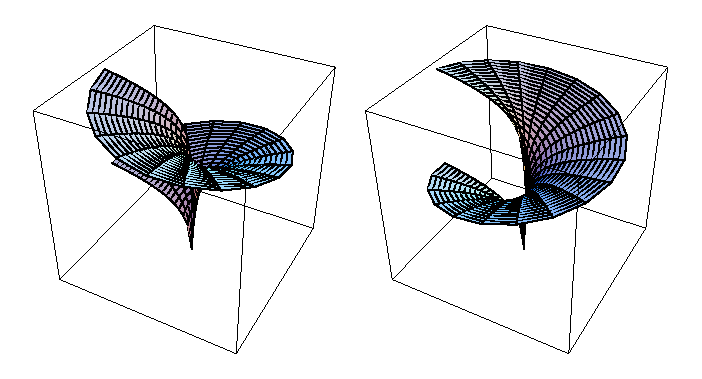
\includegraphics[width=0.6\textwidth]{fcv/analytic/velocity-stream-logzilogz}
      \end{center}
      \caption{The velocity potential and the stream function.}
      \label{figure velocity-stream-logzilogz}
    \end{figure}
    
    Next we find the stream lines, $\psi = c$.
    \begin{align*}
      \ln r + \theta = c
      \\
      r = \e^{c - \theta}
    \end{align*}
    These are spirals which go counter-clockwise as we follow them to the 
    origin.  See Figure~\ref{figure streamlines-logzilogz}.
    \begin{figure}[htb!]
      \begin{center}
        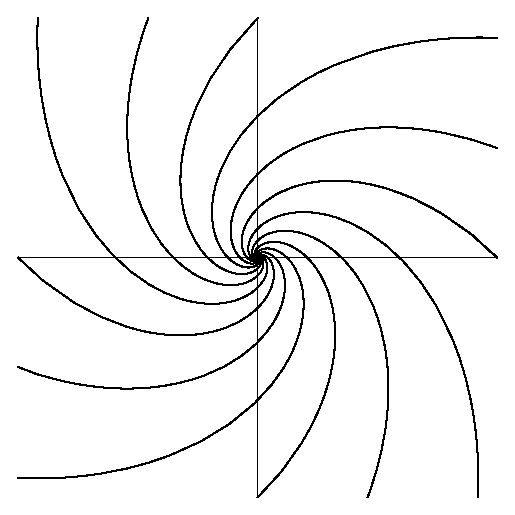
\includegraphics[width=0.25\textwidth]{fcv/analytic/streamlines-logzilogz}
      \end{center}
      \caption{The streamlines.}
      \label{figure streamlines-logzilogz}
    \end{figure}
    Next we find the velocity field.
    \begin{gather*}
      \mathbf{v} = \nabla \phi
      \\
      \mathbf{v} = \phi_r \hat{\mathbf{r}} + \frac{\phi_\theta}{r} \hat{\boldsymbol{\theta}}
      \\
      \mathbf{v} = \frac{ \hat{\mathbf{r}} }{ r } 
      - \frac{ \hat{\boldsymbol{\theta}} }{ r }
    \end{gather*}
    The velocity field is shown in the first plot of
    Figure~\ref{figure velocity-field-logzilogz}.
    We see that the fluid flows out from the origin along the spiral paths 
    of the streamlines.
    The second plot shows the direction of the velocity field.
    \begin{figure}[htb!]
      \begin{center}
        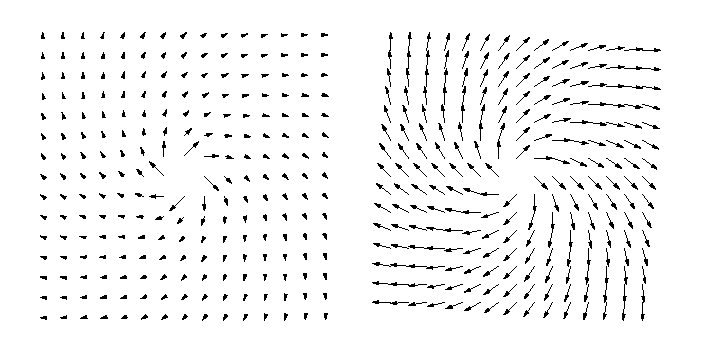
\includegraphics[width=\textwidth]{fcv/analytic/velocity-field-logzilogz}
      \end{center}
      \caption{Velocity field and velocity direction field.}
      \label{figure velocity-field-logzilogz}
    \end{figure}
    %%
    %%
  \item 
    We find the velocity potential $\phi$ and stream function $\psi$.
    \begin{gather*}
      \Phi(z) = \log(z - 1) + \log(z + 1)
      \\
      \Phi(z) = \ln |z-1| + \imath \arg(z-1) + \ln |z+1| + \imath \arg(z+1)
      \\
      \phi = \ln |z^2 - 1|, \quad \psi = \arg(z-1) + \arg(z+1)
    \end{gather*}
    The velocity potential and a branch of the stream function are plotted in 
    Figure~\ref{figure velocity-stream-logz1logz1}.
    \begin{figure}[htb!]
      \begin{center}
        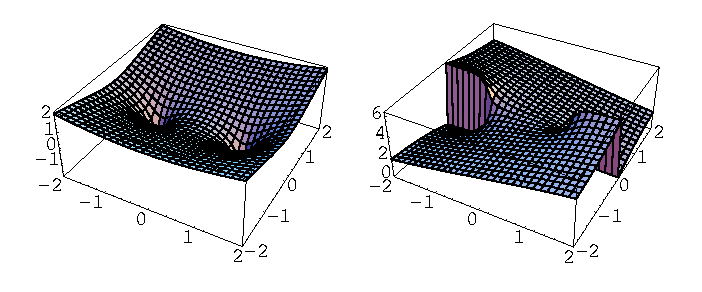
\includegraphics[width=0.7\textwidth]{fcv/analytic/velocity-stream-logz1logz1}
      \end{center}
      \caption{The velocity potential and the stream function.}
      \label{figure velocity-stream-logz1logz1}
    \end{figure}
    
    The stream lines, $\arg(z-1) + \arg(z+1) = c$,
    are plotted in Figure~\ref{figure streamlines-logz1logz1}.
    \begin{figure}[htb!]
      \begin{center}
        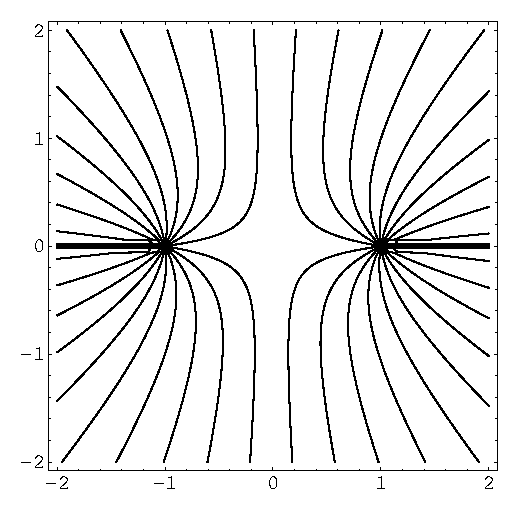
\includegraphics[width=0.5\textwidth]{fcv/analytic/streamlines-logz1logz1}
      \end{center}
      \caption{The streamlines.}
      \label{figure streamlines-logz1logz1}
    \end{figure}

    Next we find the velocity field.
    \begin{gather*}
      \mathbf{v} = \nabla \phi
      \\
      \mathbf{v} = \frac{ 2 x (x^2 + y^2 - 1) }
      { x^4 + 2 x^2 (y^2 - 1) + (y^2 + 1)^2 } \hat{\mathbf{x}}
      + \frac{ 2 y (x^2 + y^2 + 1) }
      { x^4 + 2 x^2 (y^2 - 1) + (y^2 + 1)^2 } \hat{\mathbf{y}}
    \end{gather*}
    The velocity field is shown in the first plot of
    Figure~\ref{figure velocity-field-logz1logz1}.
    The fluid is flowing out of sources at $z = \pm 1$.  The second plot shows
    the direction of the velocity field.
    \begin{figure}[htb!]
      \begin{center}
        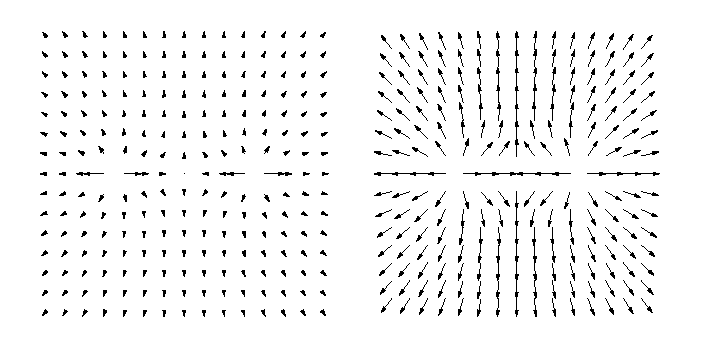
\includegraphics[width=\textwidth]{fcv/analytic/velocity-field-logz1logz1}
      \end{center}
      \caption{Velocity field and velocity direction field.}
      \label{figure velocity-field-logz1logz1}
    \end{figure}
  \end{enumerate}
\end{Solution}





\begin{Solution}
  \label{solution classify z z2+1}
\begin{enumerate}
\item 
  \begin{enumerate}
  \item 
    We factor the denominator to see that there are first order poles at 
    $z = \pm \imath$.
    \[
    \frac{z}{z^2 + 1} = \frac{z}{(z - \imath) (z + \imath)}
    \]
    Since the function behaves like $1/z$ at infinity, it is analytic there.
  \item 
    The denominator of $1 / \sin z$ has first order zeros at $z = n \pi$,
    $n \in \mathbb{Z}$.
    Thus the function has first order poles at these locations.
    Now we examine the point at infinity with the change of variables
    $z = 1 / \zeta$.
    \[
    \frac{1}{\sin z} = \frac{1}{ \sin(1 / \zeta)} = \frac{\imath 2}{\e^{\imath / \zeta} - \e^{-\imath / \zeta}}
    \]
    We see that the point at infinity is a singularity of the function.
    Since the denominator grows exponentially, there is no multiplicative
    factor of $\zeta^n$ that will make the function analytic at $\zeta = 0$.  We conclude
    that the point at infinity is an essential singularity.  Since there is
    no deleted neighborhood of the point at infinity that does contain
    first order poles at the locations $z = n \pi$, the point at infinity is
    a non-isolated singularity.
  \item 
    \[
    \log \left( 1 + z^2 \right) = \log(z + \imath) + \log(z - \imath)
    \]
    There are branch points at $z = \pm \imath$.  Since the argument of the logarithm
    is unbounded as $z \to \infty$ there is a branch point at infinity as well.
    Branch points are non-isolated singularities.
  \item 
    \[
    z \sin(1/z) = \frac{1}{2} z \left( \e^{\imath / z} + \e^{\imath / z} \right)
    \]
    The point $z = 0$ is a singularity.  Since the function grows 
    exponentially at $z = 0$.  There is no multiplicative factor of $z^n$
    that will make the function analytic.  Thus $z = 0$ is an essential
    singularity.
    
    There are no other singularities in the finite complex plane.  We examine
    the point at infinity.
    \[
    z \sin \left( \frac{1}{z} \right) 
    = \frac{1}{\zeta} \sin \zeta
    \]
    The point at infinity is a singularity.  We take the limit $\zeta \to 0$ to 
    demonstrate that it is a removable singularity.
    \[
    \lim_{\zeta \to 0} \frac{\sin \zeta}{\zeta} 
    = \lim_{\zeta \to 0} \frac{\cos \zeta}{1} 
    = 1
    \]
  \item 
    \[
    \frac{ \tan^{-1}(z)}{z \sinh^2(\pi z)}
    = \frac{ \imath \log \left( \frac{\imath + z}{\imath - z} \right) }{2 z \sinh^2(\pi z)}
    \]
    There are branch points at $z = \pm \imath$ due to the logarithm.  These are 
    non-isolated singularities.  Note that $\sinh(z)$ has first order zeros
    at $z = \imath n \pi$, $n \in \mathbb{Z}$.  The arctangent has a first order zero
    at $z = 0$.
    Thus there is a second order pole at 
    $z = 0$.  There are second order poles at $z = \imath n$, 
    $n \in \mathbb{Z} \setminus \{0\}$ due to the hyperbolic sine.  Since the hyperbolic
    sine has an essential singularity at infinity, the function has 
    an essential singularity at infinity as well.  The point at infinity
    is a non-isolated singularity because there is no neighborhood of infinity
    that does not contain second order poles.
  \end{enumerate}
\item 
  \begin{enumerate}
  \item 
    $(z - \imath) \e^{1 / (z - 1)}$ has a simple zero at $z = \imath$ and an isolated 
    essential singularity at $z = 1$.
  \item 
    \[
    \frac{\sin(z - 3)}{(z - 3) (z + \imath)^6}
    \]
    has a removable singularity at $z = 3$, a pole of order 6 at $z = - \imath$ 
    and an essential singularity at $z_\infty$.
  \end{enumerate}
\end{enumerate}
\end{Solution}









\raggedbottom
}
